\chapter{Eingang/Ausgang}

\renewcommand{\thepage}{\arabic{page}}
\setcounter{page}{1}

\section{Ausgang}
\label{ref:ModelElementDispose}

\begin{wrapfigure}{l}{2.5cm}
\vspace{-22pt}
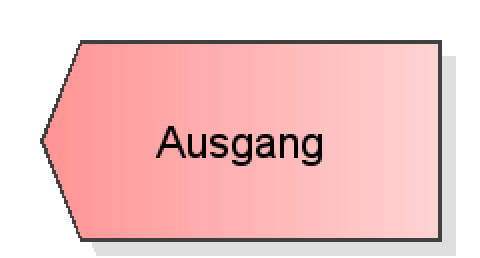
\includegraphics[width=2cm]{imageModelElementDispose.png}
\vspace{-22pt}
\end{wrapfigure}

Siehe auch Abschnitt \textbf{Station: Ausgang} im Lehrbuch.

In ein Ausgang-Element können beliebig viele Kanten einlaufen, es laufen aus diesem Element jedoch keine Kanten mehr aus.
Das Ausgang stellt die letzte Station eines Kunden in dem Warteschlangensystem dar. An dieser Station verlässt der Kunde
das System, eine weitere Verarbeitung ist danach nicht mehr möglich. Alle Wege der Kunden müssen in solch einem Element enden.

\subsection*{Einstellungen}

Für das Ausgang-Element kann ein Name eingestellt werden. Dieser hat jedoch keine weitere Bedeutung, sondern wird lediglich
in der Komponente auf der Zeichenfläche angezeigt.

Zusätzlich kann eingestellt werden, dass ein Ausgang-Element als Notausgang verwendet werden soll: Befindet sich das Element
in diesem Modus, so wird die Simulation abgebrochen, so bald an der Station ein Kunde eintrifft.


\section{Datenbankquelle}
\label{ref:ModelElementSourceDB}

\begin{wrapfigure}{l}{2.5cm}
\vspace{-22pt}
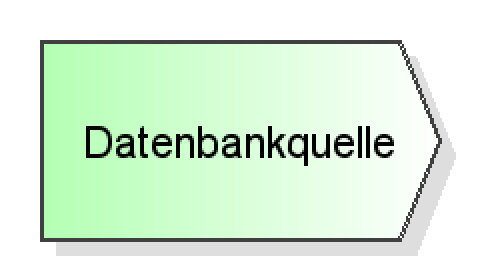
\includegraphics[width=2cm]{imageModelElementSourceDB.png}
\vspace{-22pt}
\end{wrapfigure}

Siehe auch Abschnitt \textbf{Tabellenquellen} im Lehrbuch.

Die Quelle stellt den Startpunkt der Bewegung eines Kunden durch das System dar.
Ein Simulationsmodell kann aus einer oder mehreren Quellen bestehen.
Eine datenbankbasierte Quelle erstellt Kundenankünfte nicht basierend auf
Zeitabständen oder ähnlichem, sondern lädt die konkreten Zeitpunkte aus einer
Tabelle einer Datenbank.

\subsection*{Einstellungen}

Der Name der Datenbankquelle besitzt keine Bedeutung für die Simulation.
Bei jeder Datenbankquelle müssen neben den Einstellungen zur Verbindung mit
der Datenbank der Name der Tabelle, aus der die Ankünfte geladen werden sollen
sowie die Spalten für die Ankunftszeiten (in Sekunden), die jeweiligen Kundentypen
und optional für Kundendaten angegeben werden. Des weiteren muss angegeben werden,
welche Kundentypen in der Tabelle berücksichtigt werden sollen.

Bei der Kundendaten-Spalte handelt es sich um eine Tabellenspalte die Ausdrücke
der Form ,,\texttt{ClientData(1)=Formel}'', ,,\texttt{ClientData('Schlüssel')=Textwert}"
oder \texttt{w=Formel} enthält. (Statt \texttt{w} stehen auch \texttt{t}, \texttt{p},
\texttt{wCosts}, \texttt{tCosts} und \texttt{pCosts} zur Verfügung.)
Es können auch mehrere Kundendatenfelder gesetzt werden.
Die Ausdrücke müssen dann innerhalb der Zelle durch \textbf{Tabulatoren} getrennt werden.

Siehe auch die Erklärungen auf der Hilfeseite zur Tabellenquelle (siehe Seite \pageref{ref:ModelElementSourceTable}) -Station.


\section{Excel-DDE-Quelle}
\label{ref:ModelElementSourceDDE}

\begin{wrapfigure}{l}{2.5cm}
\vspace{-22pt}
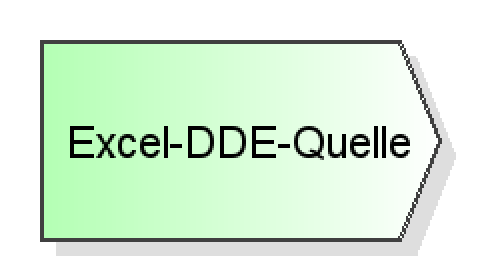
\includegraphics[width=2cm]{imageModelElementSourceDDE.png}
\vspace{-22pt}
\end{wrapfigure}

Siehe auch Abschnitt \textbf{Tabellenquellen} im Lehrbuch.

Die Quelle stellt den Startpunkt der Bewegung eines Kunden durch das System dar.
Ein Simulationsmodell kann aus einer oder mehreren Quellen bestehen.
Eine DDE-tabellenbasierte Quelle erstellt Kundenankünfte nicht basierend auf
Zeitabständen oder ähnlichem, sondern lädt die konkreten Zeitpunkte per DDE
aus einer Tabelle.

\subsection*{Einstellungen}

Der Name der Excel-DDE-Quelle besitzt keine Bedeutung für die Simulation.
Bei jeder Excel-DDE-Quelle müssen die \textbf{DDE-Verbindungseinstellungen}
(Arbeitsmappe, Tabelle und Startzelle) über die die Ankünfte geladen werden sollen,
sowie die \textbf{Liste der Kundentypnamen},
für die Ankünfte aus der Tabelle geladen werden sollen, angegeben werden.

\textbf{Aufbau der Tabelle:}~\\
Die Tabelle muss aus mindestens zwei Spalten bestehen. Die erste Spalte enthält die Ankunftszeitpunkte
der Kunden gemessen in Sekunden beginnend mit dem Start der Simulation oder aber die Abstände
der Ankünfte der Kunden untereinander ebenfalls gemessen in Sekunden. Die zweite Spalte
enthält zu jedem Ankunftszeitpunkt den Namen des Kundentyps des Kunden, der an dem
angegebenen Zeitpunkt eintreffen soll. Zeilen, bei denen der angegebene Kundentyp
nicht in der im Element eingestellten Liste der Kundentypnamen enthalten ist, werden ignoriert.
Alle weiteren Spalten enthalten optional Ausdrücke der folgenden Formen:

\begin{itemize}
  \item \texttt{ClientData(nr)=Formel}<br>
  Weist an das numerische Kundendatenfeld mit dem Index \texttt{nr} das Ergebnis der
  Auswertung von \texttt{Formel} zu. 
  \item \texttt{ClientData('Schlüssel')=Textwert}<br>
  Weist an \texttt{Schlüssel} den Wert \texttt{Textwert} zu. 
  \item \texttt{w=Formel}<br>
  Stellt den Wartezeitzähler des Kunden initial auf das Ergebnis der
  Auswertung von \texttt{Formel}.   
  \item \texttt{t=Formel}<br>
  Stellt den Transportzeitzähler des Kunden initial auf das Ergebnis der
  Auswertung von \texttt{Formel}. 
  \item \texttt{p=Formel}<br>
  Stellt den Bedienzeitzähler des Kunden initial auf das Ergebnis der
  Auswertung von \texttt{Formel}. 
  \item \texttt{wCosts=Formel}<br>
  Stellt die wartezeitabhängigen Kosten initial auf das Ergebnis der
  Auswertung von \texttt{Formel}. 
  \item \texttt{tCosts=Formel}<br>
  Stellt die transportzeitabhängigen Kosten initial auf das Ergebnis der
  Auswertung von \texttt{Formel}. 
  \item \texttt{pCosts=Formel}<br>
  Stellt die bedienzeitabhängigen Kosten initial auf das Ergebnis der
  Auswertung von \texttt{Formel}. 
\end{itemize}

Auf diese Weise können in den neu erstellten Kundenobjekten direkt kundenspezifische Daten
hinterlegt werden. 


\section{Mehrfachquelle}
\label{ref:ModelElementSourceMulti}

\begin{wrapfigure}{l}{2.5cm}
\vspace{-22pt}
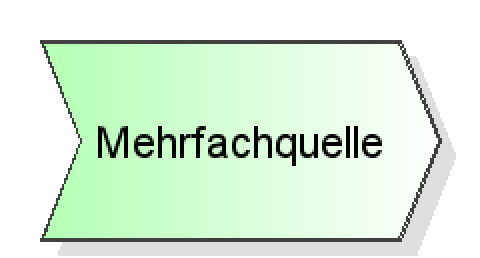
\includegraphics[width=2cm]{imageModelElementSourceMulti.png}
\vspace{-22pt}
\end{wrapfigure}

Siehe auch Abschnitt \textbf{Tabellenquellen} im Lehrbuch.

Die Mehrfachquelle stellt den Startpunkt der Bewegung eines Kunden durch das System dar.
Ein Simulationsmodell kann aus einer oder mehreren Quellen oder Mehrfachquellen bestehen.

\subsection*{Einstellungen}

Der Name der Mehrfachquelle besitzt keine weitere Bedeutung für die Simulation.

Pro Kunden-Teilquelle können folgende Eigenschaften eingestellt werden: 

Zunächst muss ein \textbf{Name} für den Typ der zu generierenden Kunden angegeben werden.
Der Dialog besitzt eine Reihe von Registerkarten, über die die verschiedenen Eigenschaften
der Kundenquelle konfiguriert werden können:

\subsubsection*{Zwischenankunftszeiten}

In Bezug auf die Zwischenankunftszeiten kann eingestellt werden, ob diese gemäß einer
\textbf{Verteilung}, gemäß einem \textbf{Ausdruck}, über einen \textbf{Zeitplan}, über eine
\textbf{Freigabebedingung} bzw. einen \textbf{Schwellenwert}, über ein oder mehrere
\textbf{Signale}, über eine \textbf{Anzahl pro Intervall}, über \textbf{Zwischenankunftszeiten pro Intervall}
oder über vorgegebene \textbf{Zahlenwerte}, die Ankunftszeitpunkte oder Zwischenankunftszeiten
repräsentieren bestimmt werden sollen.

\subsubsection*{Batch-Größe}

Über die Batch-Größe kann zusätzlich
angegeben werden, dass pro Ankunft nicht ein einzelner Kunde, sondern zeitgleich jeweils
mehrere Kunden eintreffen sollen. Dabei kann eingestellt werden, dass immer gleich
viele Kunden pro Ankunft eintreffen (feste Batch-Größe) oder aber es kann eine Verteilung
der Raten, gemäß denen die jeweilige Größe des Ankunfts-Batches bestimmt werden soll,
angegeben werden.
Die Zwischenankunftszeiten beziehen sich im Fall von Batch-Ankünften auf die Abstände von
einem Batch zum nächsten. Treffen z.B. immer 3er Batche mit einer mittleren Zwischenankunftszeit
von 2 Minuten ein, so trifft umgerechnet im Mittel alle 40 Sekunden ein Kunde ein.

\subsubsection*{Anzahl an Ankünften}

Im Normalfall generiert eine Quelle gemäß der Zwischenankunftszeitenverteilung fortwährend
weitere Ankünfte bis die Gesamtanzahl an geplanten Ankünften erreicht wurden bzw. die Simulation beendet wurde.
Es kann jedoch auch eingestellt werden, dass die Quelle bereits zu einem früheren Zeitpunkt,
d.h. nach einer konkret einstellbaren Anzahl an Ankünften, das Generieren weiterer Ankünfte einstellt.
Alternativ kann auch eine maximale Anzahl an zu generierenden Kunden vorgegeben werden.
Werden keine Batch-Ankünfte versendet, so entspricht die Anzahl an Ankunftsereignissen der
Anzahl an Kunden. Bei Batch-Ankünften treffen mehr Kunden ein, als es Ankunftsereignisse gibt.

\subsubsection*{Startzeitpunkt}

Normalerweise beginnt die Quelle sofort nach Start der Simulation mit der Generierung von
Ankünften. Durch die Festlegung eines positiven Startzeitpunktes kann jedoch eingestellt
werden, dass die erste Zwischenankunftszeit (an deren Ende die erste Kundenankunft steht) erst
zu einem späteren Zeitpunkt beginnt.

Bei der Erzeugung von Ankünften mit bestimmten Zwischenankunftszeiten (definiert über eine Verteilung
oder einen Rechenausdruck) beginnt im Normalfall die erste Zwischenankunftszeit ab dem Startzeitpunkt.
Die tatsächliche erste Ankunft erfolgt dann zum Zeitpunkt Startzeitpunkt+Zwischenankunftszeit. Über
die Option \textbf{Erste Ankunft zum Zeitpunkt 0} kann eingestellt werden, dass bereits direkt zum
Startzeitpunkt die erste Ankunft erfolgen soll.

\subsubsection*{Zuweisung von Kundenvariablen}

Auf dieser Registerkarte können Kundenvariablen vom Typ \texttt{ClientData(nr)} eingetragen werden,
die jedem neu erstellten Kunden automatisch zugewiesen werden sollen.

\subsubsection*{Zuweisung von Texten}

Auf dieser Registerkarte können Textzuweisungen vom Typ Schlüssel:=Text eingetragen werden,
die jedem neu erstellten Kunden automatisch zugewiesen werden sollen.

\subsubsection*{Modus der Teil-Quellen}

Es kann eingestellt werden, ob alle Teil-Quellen gleichzeitig aktiv sein sollen, d.h. die Mehrfachquelle
so agiert, als würde sie aus mehreren einzelnen, unabhängigen Kundenquellen bestehen, oder ob die Teil-Quellen
jeweils reihum zum Zuge kommen sollen. Im zweiteren Modus müssen die Zwischenankunftszeiten für die Teil-Quellen
durchgängig über Wahrscheinlichkeitsverteilungen oder Rechenausdrücke definiert sein.

\subsubsection*{Gesamtanzahl der generierten Kunden begrenzen}

Optional kann eine Grenze für die Anzahl an zu generierenden Kunden über alle Teil-Quellen hinweg
eingestellt werden.

\subsection*{Kundentypen laden}

Sollen in einem Modell sehr viele Kundentypen verwendet werden, so können über diese Funktion mehrere
Kundentypen aus einer Tabelle geladen werden. Jede Tabellenzeile enthält dabei die Daten zu einem Kundentyp.

Die erste Spalte muss den Namen des Kundentyps angeben, die zweite die Definition der Zwischenankunftszeiten.
Dabei können die Zwischenankunftszeiten entweder über einen Rechenausdruck oder über die Definition einer
Verteilungsfunktion festgelegt werden. Das Format der Verteilungsfunktionsdefinition ist in dem pdf-Dokument
"Distribution XML reference for Warteschlangensimulator'' dokumentiert. Auf diese beiden Spalten können beliebig
viele weitere Spalten mit folgenden Inhalten folgen:

\begin{itemize}
  \item \texttt{batch=}<br>
  Gibt die Ankunfts-Batch-Größe an. Es kann entweder eine positive Ganzzahl angegeben werden oder eine Reihe von
  durch ,,;'' getrennte Werte der Form \texttt{Größe=Rate} zur Definition verschiedener Raten für verschiedene Batch-Größen. 
  \item \texttt{count=}<br>
  Gibt die Gesamtanzahl an Ankunftsereignissen an. 
  \item \texttt{start=}<br>
  Gibt den Start der ersten Zwischenankunftszeit an. 
\end{itemize}

Außerdem stehen die Zuweisungen, die an einer Tabellenquelle (siehe Seite \pageref{ref:ModelElementSourceTable}) genutzt werden können, zur Verfügung.


\section{Quelle}
\label{ref:ModelElementSource}

\begin{wrapfigure}{l}{2.5cm}
\vspace{-22pt}
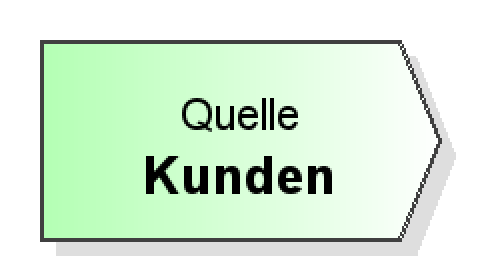
\includegraphics[width=2cm]{imageModelElementSource.png}
\vspace{-22pt}
\end{wrapfigure}

Siehe auch Abschnitt \textbf{Station: Kundenquelle} im Lehrbuch.

Die Quelle stellt den Startpunkt der Bewegung eines Kunden durch das System dar.
Ein Simulationsmodell kann aus einer oder mehreren Quellen bestehen.

\subsection*{Einstellungen}

Der \textbf{Name} der Quelle bestimmt zugleich den Namen der Kunden, die ihr entspringen.
Der Dialog besitzt eine Reihe von Registerkarten, über die die verschiedenen Eigenschaften
der Kundenquelle konfiguriert werden können:

\subsubsection*{Zwischenankunftszeiten}

In Bezug auf die Zwischenankunftszeiten kann eingestellt werden, ob diese gemäß einer
\textbf{Verteilung}, gemäß einem \textbf{Ausdruck}, über einen \textbf{Zeitplan}, über eine
\textbf{Freigabebedingung} bzw. einen \textbf{Schwellenwert}, über ein oder mehrere
\textbf{Signale}, über eine \textbf{Anzahl pro Intervall}, über \textbf{Zwischenankunftszeiten pro Intervall}
oder über vorgegebene \textbf{Zahlenwerte}, die Ankunftszeitpunkte oder Zwischenankunftszeiten
repräsentieren bestimmt werden sollen.

\subsubsection*{Batch-Größe}

Über die Batch-Größe kann zusätzlich
angegeben werden, dass pro Ankunft nicht ein einzelner Kunde, sondern zeitgleich jeweils
mehrere Kunden eintreffen sollen. Dabei kann eingestellt werden, dass immer gleich
viele Kunden pro Ankunft eintreffen (feste Batch-Größe) oder aber es kann eine Verteilung
der Raten, gemäß denen die jeweilige Größe des Ankunfts-Batches bestimmt werden soll,
angegeben werden.
Die Zwischenankunftszeiten beziehen sich im Fall von Batch-Ankünften auf die Abstände von
einem Batch zum nächsten. Treffen z.B. immer 3er Batche mit einer mittleren Zwischenankunftszeit
von 2 Minuten ein, so trifft umgerechnet im Mittel alle 40 Sekunden ein Kunde ein.

\subsubsection*{Anzahl an Ankünften}

Im Normalfall generiert eine Quelle gemäß der Zwischenankunftszeitenverteilung fortwährend
weitere Ankünfte bis die Gesamtanzahl an geplanten Ankünften erreicht wurden bzw. die Simulation beendet wurde.
Es kann jedoch auch eingestellt werden, dass die Quelle bereits zu einem früheren Zeitpunkt,
d.h. nach einer konkret einstellbaren Anzahl an Ankünften, das Generieren weiterer Ankünfte einstellt.
Alternativ kann auch eine maximale Anzahl an zu generierenden Kunden vorgegeben werden.
Werden keine Batch-Ankünfte versendet, so entspricht die Anzahl an Ankunftsereignissen der
Anzahl an Kunden. Bei Batch-Ankünften treffen mehr Kunden ein, als es Ankunftsereignisse gibt.

\subsubsection*{Startzeitpunkt}

Normalerweise beginnt die Quelle sofort nach Start der Simulation mit der Generierung von
Ankünften. Durch die Festlegung eines positiven Startzeitpunktes kann jedoch eingestellt
werden, dass die erste Zwischenankunftszeit (an deren Ende die erste Kundenankunft steht) erst
zu einem späteren Zeitpunkt beginnt.

Bei der Erzeugung von Ankünften mit bestimmten Zwischenankunftszeiten (definiert über eine Verteilung
oder einen Rechenausdruck) beginnt im Normalfall die erste Zwischenankunftszeit ab dem Startzeitpunkt.
Die tatsächliche erste Ankunft erfolgt dann zum Zeitpunkt Startzeitpunkt+Zwischenankunftszeit. Über
die Option \textbf{Erste Ankunft zum Zeitpunkt 0} kann eingestellt werden, dass bereits direkt zum
Startzeitpunkt die erste Ankunft erfolgen soll.

\subsubsection*{Zuweisung von Kundenvariablen}

Auf dieser Registerkarte können Kundenvariablen vom Typ \texttt{ClientData(nr)} eingetragen werden,
die jedem neu erstellten Kunden automatisch zugewiesen werden sollen.

\subsubsection*{Zuweisung von Texten}

Auf dieser Registerkarte können Textzuweisungen vom Typ Schlüssel:=Text eingetragen werden,
die jedem neu erstellten Kunden automatisch zugewiesen werden sollen.


\section{Speichern+Ausgang}
\label{ref:ModelElementDisposeWithTable}

\begin{wrapfigure}{l}{2.5cm}
\vspace{-22pt}
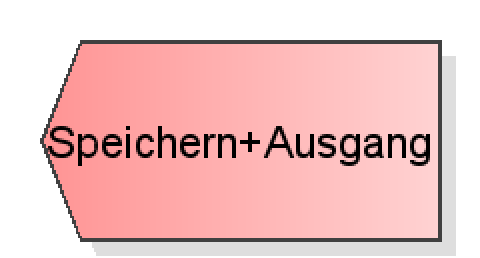
\includegraphics[width=2cm]{imageModelElementDisposeWithTable.png}
\vspace{-22pt}
\end{wrapfigure}

In ein Ausgang-Element können beliebig viele Kanten einlaufen, es laufen aus diesem Element jedoch keine Kanten mehr aus.
Das Ausgang stellt die letzte Station eines Kunden in dem Warteschlangensystem dar. An dieser Station verlässt der Kunde
das System, eine weitere Verarbeitung ist danach nicht mehr möglich. Alle Wege der Kunden müssen in solch einem Element enden.

Ein Speichern+Ausgang-Element erfasst die einzelnen Kunden vor dem Verlassen des Systems in einer Tabelle. Auf diese Art
generierte Tabellen könne an Tabellen-Quellen (siehe Seite \pageref{ref:ModelElementSourceTable}) verwendet werden, um so die
Kunden, die das aktuelle System verlassen haben, als Eingangsstrom in einem anderen Modell zu verwenden.

\subsection*{Einstellungen}

Bei einem Speichern+Ausgang-Element muss eine Datei angegeben werden, in der die Kunden vor dem verlassen des Systems erfasst werden.

Für das Ausgang-Element kann ein Name eingestellt werden. Dieser hat jedoch keine weitere Bedeutung, sondern wird lediglich
in der Komponente auf der Zeichenfläche angezeigt.

Zusätzlich kann eingestellt werden, dass ein Ausgang-Element als Notausgang verwendet werden soll: Befindet sich das Element
in diesem Modus, so wird die Simulation abgebrochen, so bald an der Station ein Kunde eintrifft.

\subsection*{Hinweis}

Die an dieser Station erzeugten Tabellen können über den <a hrref="ProcessClientOutputTable.html">Ausgabetabelle aufbereiten</a>-Dialog
in normale Tabellen umgewandelt werden.


\section{Tabellenquelle}
\label{ref:ModelElementSourceTable}

\begin{wrapfigure}{l}{2.5cm}
\vspace{-22pt}
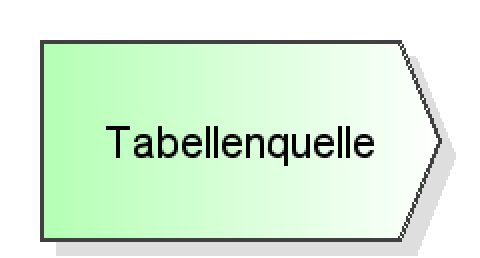
\includegraphics[width=2cm]{imageModelElementSourceTable.png}
\vspace{-22pt}
\end{wrapfigure}

Siehe auch Abschnitt \textbf{Tabellenquellen} im Lehrbuch.

Die Quelle stellt den Startpunkt der Bewegung eines Kunden durch das System dar.
Ein Simulationsmodell kann aus einer oder mehreren Quellen bestehen.
Eine tabellenbasierte Quelle erstellt Kundenankünfte nicht basierend auf
Zeitabständen oder ähnlichem, sondern lädt die konkreten Zeitpunkte aus einer
Tabelle.

\subsection*{Einstellungen}

Der Name der Tabellenquelle besitzt keine Bedeutung für die Simulation.
Bei jeder Tabellenquelle müssen der \textbf{Dateiname der Tabelle}, aus
der die Ankünfte geladen werden sollen, sowie die \textbf{Liste der Kundentypnamen},
für die Ankünfte aus der Tabelle geladen werden sollen, angegeben werden.

Soll an einer Tabellenquelle eine Tabelle \textbf{direkt ohne Vorverarbeitung}
verwendet werden, so muss über den über das Zahnrad-Symbol rechts neben dem Eingabefeld
für den Dateinamen der Tabelle aufrufbaren Dialog die Bedeutung der Tabellen konfiguriert werden.
Im Falle einer \textbf{bereits vorab aufbereiteten} Tabelle ist dies nicht notwendig.

\textbf{Aufbau einer aufbereiteten Tabelle:}~\\
Die Tabelle muss aus mindestens zwei Spalten bestehen. Die erste Spalte enthält die Ankunftszeitpunkte
der Kunden gemessen in Sekunden beginnend mit dem Start der Simulation oder aber die Abstände
der Ankünfte der Kunden untereinander ebenfalls gemessen in Sekunden. Die zweite Spalte
enthält zu jedem Ankunftszeitpunkt den Namen des Kundentyps des Kunden, der an dem
angegebenen Zeitpunkt eintreffen soll. Zeilen, bei denen der angegebene Kundentyp
nicht in der im Element eingestellten Liste der Kundentypnamen enthalten ist, werden ignoriert.
Alle weiteren Spalten enthalten optional Ausdrücke der folgenden Formen:

\begin{itemize}
  \item \texttt{ClientData(nr)=Formel}<br>
  Weist an das numerische Kundendatenfeld mit dem Index \texttt{nr} das Ergebnis der
  Auswertung von \texttt{Formel} zu. 
  \item \texttt{ClientData('Schlüssel')=Textwert}<br>
  Weist an \texttt{Schlüssel} den Wert \texttt{Textwert} zu. 
  \item \texttt{w=Formel}<br>
  Stellt den Wartezeitzähler des Kunden initial auf das Ergebnis der
  Auswertung von \texttt{Formel}.   
  \item \texttt{t=Formel}<br>
  Stellt den Transportzeitzähler des Kunden initial auf das Ergebnis der
  Auswertung von \texttt{Formel}. 
  \item \texttt{p=Formel}<br>
  Stellt den Bedienzeitzähler des Kunden initial auf das Ergebnis der
  Auswertung von \texttt{Formel}. 
  \item \texttt{wCosts=Formel}<br>
  Stellt die wartezeitabhängigen Kosten initial auf das Ergebnis der
  Auswertung von \texttt{Formel}. 
  \item \texttt{tCosts=Formel}<br>
  Stellt die transportzeitabhängigen Kosten initial auf das Ergebnis der
  Auswertung von \texttt{Formel}. 
  \item \texttt{pCosts=Formel}<br>
  Stellt die bedienzeitabhängigen Kosten initial auf das Ergebnis der
  Auswertung von \texttt{Formel}. 
\end{itemize}

Auf diese Weise können in den neu erstellten Kundenobjekten direkt kundenspezifische Daten
hinterlegt werden. 

\textbf{Hinweis:}
Über die Schaltfläche rechts neben der Eingabezeile für die Tabellendatei kann der
Tabelle für Tabellenquelle aufbereiten -Dialog
aufgerufen werden, in dem Tabellen in normaler Spaltenform in Tabellen in dem oben
beschriebenen Format umgewandelt werden können.





\chapter{Verarbeitung}

\section{Bedienstation}
\label{ref:ModelElementProcess}

\begin{wrapfigure}{l}{2.5cm}
\vspace{-22pt}
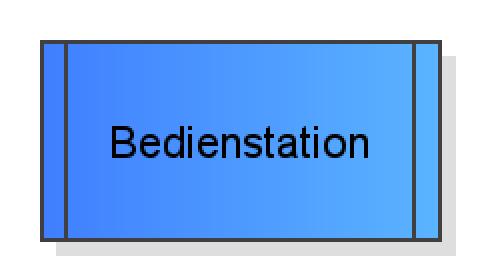
\includegraphics[width=2cm]{imageModelElementProcess.png}
\vspace{-22pt}
\end{wrapfigure}

Siehe auch Abschnitt \textbf{Station: Bedienstation} im Lehrbuch.

Die Bedienstation ist das zentrale Element eines jeden Simulationsmodells. In einer Bedienstation warten Kunden darauf,
dass ein Bediener verfügbar wird, und werden dann von diesem Bediener eine bestimmte Zeit lang bedient. Kunden, deren
(optionale) Wartezeittoleranz überschritten wurde, werden zu Warteabbrechern und geben das Warten auf, ohne bedient
worden zu sein. Ein Bediener kann (ebenfalls optional) nach der Bedienung in eine Nachbearbeitungszeit gehen, bevor
er wieder bereit ist, den nächsten Kunden zu bedienen.

Es kann angegeben werden, dass statt eines Bedieners mehrere Bediener optional aus mehreren verschiedenen Gruppen zur Bedienung
eines Kunden benötigt werden.

Des Weiteren kann eingestellt werden, dass die Kunden nicht einzeln, sondern in Gruppen bedient werden. In diesem Fall
beziehen sich die notwendigen Anzahlen an Bedienern darauf, eine ganze Gruppe zu bedienen.

\subsection*{Einstellungen}

\subsubsection*{Name}

Der Name des Bedienstation-Elements hat keine weitere Bedeutung.

\subsubsection*{Bedienzeiten}

Auf dieser Dialogseite kann die Wahrscheinlichkeitsverteilung für die Bedienzeiten oder der Ausdruck gemäß
dessen die Bedienzeiten der Kunden bestimmt werden eingestellt werden. Optional
kann hier für jeden Kundentyp eine individuelle Verteilung bzw. ein individueller Ausdruck hinterlegt werden.

\textbf{Hinweis zu individuellen Bedienzeiten und Batch-Verarbeitung:}~\\
Prinzipiell widersprechen sich pro Kundentyp individuelle Bedienzeiten und die gleichzeitige Bedienung von mehreren Kunden
(von möglicherweise verschiedenen Typen). Dennoch kann dies in der Simulation verwendet werden. In diesem Fall wird für jeden
in dem Batch enthaltenen Kundentyp eine Bedienzeit gemäß der vorgegebenen Verteilung bestimmt. Diese Bedienzeit gilt dann
für alle in dem Batch enthaltenen Kunden des jeweiligen Kundentyps. Die Ressourcen werden so lange belegt, bis das
Maximum der Bedienzeiten der enthaltenen Kundentypen erreicht ist.

\subsubsection*{Rüstzeiten}

Auf dieser Dialogseite können zusätzliche Zeiten, die zwischen der Bedienung gleich oder - was meist der Fall ist -
Kunden verschiedener Typen auftreten definiert werden. Diese für jeden Kundentyp-Übergang optionalen Rüstzeiten
können jeweils entweder über eine Wahrscheinlichkeitsverteilung oder einen Ausdruck definiert werden.

\textbf{Hinweis Rüstzeiten und Batch-Verarbeitung:}~\\
Rüstzeiten und Batch-Verarbeitung können an einer Bedienstation nicht gleichzeitig
verwendet werden. Eine Bedienstation mit Rüstzeiten kann sehr wohl temporär oder permanent
zu einem Batch zusammengefasste Kunden verarbeiten, allerdings eine Batch-Bildung direkt an
der Bedienstation ist nicht möglich, da in diesem Fall nicht eindeutig zu klären wäre,
welche Rüstzeit jeweils zum Tragen kommt.

\subsubsection*{Nachbearbeitungszeiten}

Über die optionalen Nachbearbeitungszeiten kann eine Wahrscheinlichkeitsverteilung oder ein Ausdruck angegeben werden, gemäß
dieser bzw. dessen die Bediener nach Abschluss der Bedienung eines Kunden zusätzliche Zeit benötigen, bevor sie wieder für
die Bearbeitung des nächsten Kunden zur Verfügung stehen. Optional kann auch hier für jeden Kundentyp eine individuelle Verteilung
bzw. ein individueller Ausdruck hinterlegt werden.

\textbf{Hinweis zu individuellen Nachbearbeitungszeiten und Batch-Verarbeitung:}~\\
Prinzipiell widersprechen sich pro Kundentyp individuelle Nachbearbeitungszeiten und die gleichzeitige Bedienung von mehreren Kunden
(von möglicherweise verschiedenen Typen). Dennoch kann dies in der Simulation verwendet werden. In diesem Fall wird für jeden
in dem Batch enthaltenen Kundentyp eine Nachbearbeitungszeiten gemäß der vorgegebenen Verteilung bestimmt. Die Ressourcen werden
dann nach dem Maximum der einzelnen Nachbearbeitungszeiten nach dem Ende der Bedienung freigegeben.

\subsubsection*{Wartezeittoleranzen}

Ist eingestellt, dass die Kunden nur begrenzt lange bereit sind zu warten, so wird für jeden Kunden gemäß der (global oder optional
pro Kundentyp einstellbaren) Wartezeittoleranzverteilung bzw. dem Wartezeittoleranz-Ausdruck eine Zeitspanne ermittelt, die der
Kunde zu warten bereit ist. Wird diese Zeit überschritten, so gibt der Kunde das Warten auf und verlässt das System,
ohne bedient worden zu sein.

\subsubsection*{Prioritäten und Batch-Größe}

Warten mehrere Kunden und wird ein Bediener verfügbar, so kann über die Prioritäten festgelegt werden, welcher Kunde als nächstes
bedient wird. Es wird jeweils der Kunde mit der höchsten Priorität als nächstes bedient.
"w'' gibt dabei abweichend von der sonst üblichen Belegung die bisherige Wartezeit des Kunden an der aktuellen Station an (und nicht
die gesamte bisherige Wartezeit des Kunden). Das bedeutet, dass die Formel ,,w'' für die Priorität zu einer
First-in-first-out-Warteschlange führt. ,,-w'' hätte ein Last-in-first-out-System zur Folge.

Die Batch-Größe gibt an, wie viele Kunden jeweils gleichzeitig von einem Bediener bedient werden können. Offensichtlich kann die
minimale Batch-Größe höchsten so groß wie die maximale Batch-Größe sein. Sind beide Werte identisch, so ergibt sich eine feste
Batch-Größe. Ist die minimale Batch-Größe echt kleiner als die maximale Batch-Größe, so wird nach dem Erreichen dieser Mindestanzahl
an wartenden Kunden noch eine Millisekunde abgewartet, ob weitere Kunden eintreffen. Dann werden mindestens so viele Kunden wie zuvor
eingetroffen (=minimale Batch-Größe) und höchstens so viele der dann wartenden Kunden wie die maximale Batch-Größe vorgibt, bedient. 

Im Normalfall wird die Bedienreihenfolge über die (pro Kundentyp individuell einstellbare) Prioritätsformeln festgelegt. Dies kann
jedoch zu sehr häufigen Wechseln des Kundentyps führen. Sind an einer Bedienstation Rüstzeiten beim Wechsel des Kundentyps vorgesehen,
so kann es wünschenswert sein, möglichst viele Kunden eines Typs nacheinander zu bedienen. Dies kann durch die Aktivierung des
Kampagnen-Modus erreicht werden. In diesem Fall erfolgt die Bewertung der Prioritäten zweigeteilt: Zunächst wird versucht unter den
Kunden desselben Typs, wie beim zuletzt bedienten Kunden, denjenigen mit der höchsten Priorität für die Bedienung auszusuchen.
Wartet kein Kunde desselben Typs wie der Typ des zuletzt bedienten Kunden, so wird die Prioritätsformel-basierte Suche auf alle
wartenden Kunden ausgedehnt.

\textbf{Hinweis zu variablen Batch-Größen in der Simulation:}~\\
Kunden bewegen sich grundsätzlich als individuelle Objekte durch das Warteschlangennetz. Dies hat zur Folge, dass bei Verwendung
einer variablen Batch-Größe die Bedienung der Kundengruppe theoretisch immer mit der minimalen Batch-Größe starten würde. - Auch
wenn unmittelbar die nächsten Kunden des virtuellen Batch eintreffen würden. Um dieser Tatsache Rechnung zu tragen, wartet der
Simulator nach dem Eintreffen eines Kunden, der die Anzahl an wartenden Kunden auf die minimal notwendige Batch-Größe erhöht,
noch eine Millisekunde, um so das hinzufügen von weiteren unmittelbar eintreffenden Kunden zu dem Batch zu ermöglichen.

\textbf{Hinweis zur Batch-Bedienung und zum Kampagnen-Modus:}~\\
Ein Batch umfasst mehrere Kunden; die Kunden werden dabei gemäß ihrer Prioritäten zu Bedien-Batchen zusammengestellt.
Dies bedeutet insbesondere, dass sich Kunden verschiedener Typen in einem Batch befinden können. Daher können Batche
nicht mit dem Kampagnen-Modus, der voraussetzt dass es einen eindeutigen Typ für den jeweils zuletzt bedienten
Kunden gibt, kombiniert werden. 

\subsubsection*{Bediener}

Zur Bedienung eines Kunden (bzw. eines Kunden-Batch) können mehrere Bediener aus mehreren Gruppen benötigt werden. Die Bedienung
startet nur dann, wenn gleichzeitig alle notwendigen Bediener verfügbar werden und alle gleichzeitig belegt werden können.
Darüberhinaus können mehrere Gruppenzusammenstellungs-Alternativen definiert werden. Es müssen alle Gruppen in einer der
Alternativen verfügbar sein, damit die eine Bedienung starten kann. Die Alternativen werden in der definierten Reihenfolge
auf Verfügbarkeit geprüft. 

Über die Ressourcen-Priorität kann schließlich noch festgelegt werden, mit welcher Priorität diese Bedienstation
berücksichtigt werden soll, wenn eine Ressource, die für die Bedienung der Kunden an dieser Station notwendig ist,
frei wird. Größere Werte bedeuten eine höhere Priorität bzw. eine höhere Wahrscheinlichkeit, dass diese Bedienstation
die entsprechenden Ressourcen erhält, wenn es mehrere Bedienstationen gibt, die dieselbe Ressource benötigen.

\subsubsection*{Kosten}

Auf dieser Seite kann optional eingestellt werden, welche Kosten durch die Bedienungen der Kunden entstehen.
Es handelt sich hierbei um die Kosten aus Sicht der Bedienstation. Für die Warte-, Transfer- und Bedienzeiten pro
Kunde kann in den Kundeneinstellungen pro Kundentyp ein Kostenwert hinterlegt werden. Auch können die Kosten durch
die Belegung und Bereithaltung der Ressourcen in den Ressourceneinstellungen festgelegt werden.

\subsection*{Kundentypen laden}

Sollen an einer Station sehr viele Kundentypen mit unterschiedlichen Einstellungen verwendet werden, so können über diese Funktion mehrere Kundentypdaten aus einer Tabelle geladen werden. Jede Tabellenzeile enthält dabei die Daten zu einem Kundentyp.

Die erste Spalte muss den Namen des Kundentyps angeben, die zweite die Definition der entsprechenden Zeitdauer.
Dabei können die Zeitdauern entweder über einen Rechenausdruck oder über die Definition einer
Verteilungsfunktion festgelegt werden. Das Format der Verteilungsfunktionsdefinition ist in dem pdf-Dokument
"Distribution XML reference for Warteschlangensimulator'' dokumentiert.


\section{Verzögerung}
\label{ref:ModelElementDelay}

\begin{wrapfigure}{l}{2.5cm}
\vspace{-22pt}
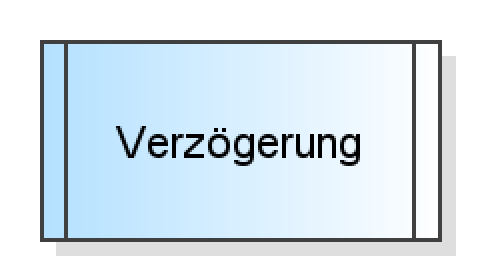
\includegraphics[width=2cm]{imageModelElementDelay.png}
\vspace{-22pt}
\end{wrapfigure}

Bei dem Durchlaufen des Verzögerung-Elements werden die Kunden für eine bestimmte, per Verteilungsfunktion oder über
einen Ausdruck festlegbare Zeitdauer verzögert. Es erfolgt keine weitere Bedienung der Kunden.

\subsection*{Einstellungen}

Der Name des Verzögerung-Elements hat keine weitere Bedeutung. Über die Verteilung oder den Ausdruck der Verzögerungszeiten kann
eingestellt werden, wie lange die einzelnen Kunden beim Durchlaufen dieses Elements warten müssen.
Es kann dabei eine globale Verteilung / ein globaler Ausdruck, die/der immer dann zur Anwendung kommt, wenn keine
kundentyp-spezifischen Daten hinterlegt sind, und optional für jeden Kundentyp ein individuelle
Verteilung bzw. ein individueller Ausdruck angegeben werden.

Sollen Kunden vor Ablauf der Verzögerungszeit über ein externes Skript-Element für die weitere Bewegung durch das System
freigegeben werden, so muss über das entsprechende Auswahlfeld aktiviert werden, dass eine entsprechende Liste für den
Skriptzugriff vorgehalten werden soll. Die Bereitstellung dieser Liste verlangsamt die Simulation, auch wenn nicht auf
sie zugegriffen wird.

\subsection*{Kundentypen laden}

Sollen an einer Station sehr viele Kundentypen mit unterschiedlichen Einstellungen verwendet werden, so können über diese Funktion mehrere Kundentypdaten aus einer Tabelle geladen werden. Jede Tabellenzeile enthält dabei die Daten zu einem Kundentyp.

Die erste Spalte muss den Namen des Kundentyps angeben, die zweite die Definition der entsprechenden Zeitdauer.
Dabei können die Zeitdauern entweder über einen Rechenausdruck oder über die Definition einer
Verteilungsfunktion festgelegt werden. Das Format der Verteilungsfunktionsdefinition ist in dem pdf-Dokument
"Distribution XML reference for Warteschlangensimulator'' dokumentiert.


\section{Verzögerung (Skript)}
\label{ref:ModelElementDelayJS}

\begin{wrapfigure}{l}{2.5cm}
\vspace{-22pt}
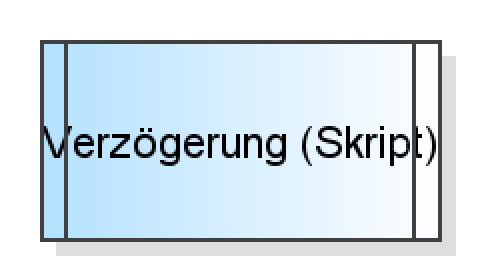
\includegraphics[width=2cm]{imageModelElementDelayJS.png}
\vspace{-22pt}
\end{wrapfigure}

Bei dem Durchlaufen des Verzögerung (Skript)-Elements werden die Kunden für eine bestimmte, per Skriptergebnis
festlegbare Zeitdauer verzögert. Es erfolgt keine weitere Bedienung der Kunden.

\subsection*{Einstellungen}

Der Name des Elements hat keine weitere Bedeutung. Über den Rückgabewert des Skriptcodes
wird jeweils bei Ankunft eines Kunden die Verzögerungszeit bestimmt.

Der Skript-Code kann beliebige Javascript-Befehle oder Java-Befehle enthalten
und kann über die zusätzlichen Javascript-Befehle bzw.
die zusätzlichen Java-Befehle auf das Simulationssystem
zugreifen. Als Rückgabewert (auszugeben über \texttt{Output.print()}) wird ein Zahlenwert
erwartet, der die Verzögerungszeit in Sekunden angibt.

Sollen Kunden vor Ablauf der Verzögerungszeit über ein externes Skript-Element für die weitere Bewegung durch das System
freigegeben werden, so muss über das entsprechende Auswahlfeld aktiviert werden, dass eine entsprechende Liste für den
Skriptzugriff vorgehalten werden soll. Die Bereitstellung dieser Liste verlangsamt die Simulation, auch wenn nicht auf
sie zugegriffen wird.





\chapter{Zuweisungen}

\section{Batch-Zähler}
\label{ref:ModelElementCounterBatch}

\begin{wrapfigure}{l}{2.5cm}
\vspace{-22pt}
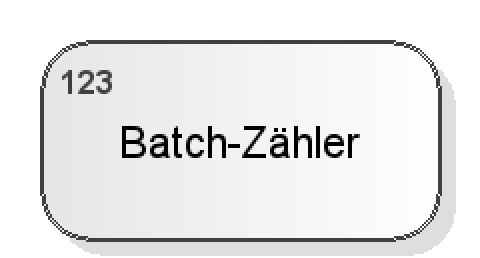
\includegraphics[width=2cm]{imageModelElementCounterBatch.png}
\vspace{-22pt}
\end{wrapfigure}

Durchlaufen Kunden mit einem zeitlichen Abstand von 0 Sekunden diese Station, so werden diese
als Batch gezählt. Die Zählung erfolgt dabei sowohl auf Batch-Basis als auch ausdifferenziert
nach Batch-Größen.

\subsection*{Einstellungen}

Der Name des Zählers definiert den Namen unter dem die Ergebnisse in der Statistik erfasst werden sollen.


\section{Bereich betreten}
\label{ref:ModelElementSectionStart}

\begin{wrapfigure}{l}{2.5cm}
\vspace{-22pt}
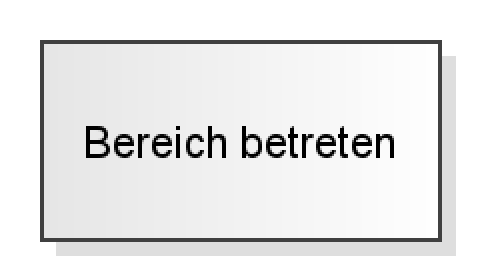
\includegraphics[width=2cm]{imageModelElementSectionStart.png}
\vspace{-22pt}
\end{wrapfigure}

Siehe auch Abschnitt \textbf{Pull-Produktion im Warteschlangensimulator} im Lehrbuch.

Bereiche ermöglichen es, in der Statistik zu erfassen, wie lange sich ein Kunde in einem bestimmten
Segment aufgehalten hat. Ein Kunde, der diese Station durchläuft, wird sofort zur nächsten Station
weitergeleitet. Allerdings wird das Verlassen der Station nicht in der Stationsstatistik erfasst,
so dass sich der Kunden aus Statistiksicht immer noch an dieser Station befindet. Erst wenn der
Kunde ein passendes Bereich verlassen-Element (siehe Seite \pageref{ref:ModelElementSectionEnd}) durchläuft,
wird er aus der Station ausgetragen.

\subsection*{Einstellungen}

Stationen dieses Typs müssen einen Namen erhalten, über den sie von
Bereich verlassen-Elementen (siehe Seite \pageref{ref:ModelElementSectionEnd}) 
aus angesprochen werden können, um signalisieren zu können, dass der
Kunde den entsprechenden Bereich jetzt verlassen hat.


\section{Bereich verlassen}
\label{ref:ModelElementSectionEnd}

\begin{wrapfigure}{l}{2.5cm}
\vspace{-22pt}
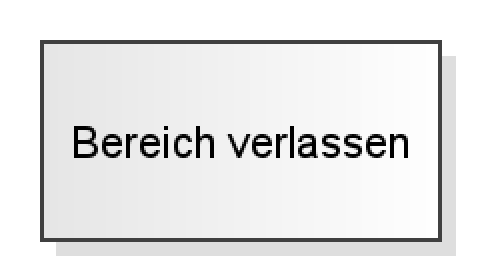
\includegraphics[width=2cm]{imageModelElementSectionEnd.png}
\vspace{-22pt}
\end{wrapfigure}

Siehe auch Abschnitt \textbf{Pull-Produktion im Warteschlangensimulator} im Lehrbuch.

Mit Hilfe eines Bereich verlassen-Elements kann einem
Bereich betreten-Element (siehe Seite \pageref{ref:ModelElementSectionStart}) 
mitgeteilt werden, dass der Kunde den betrachteten Bereich verlassen hat.

\subsection*{Einstellungen}

Der Name des Bereich verlassen-Elements hat keine weitere Bedeutung.
Es muss angegeben werden, aus welchem Bereich der Kunde beim Durchlaufen dieses
Elements ausgetragen werden soll. Hat der Kunde das zugehörige
Bereich betreten-Element (siehe Seite \pageref{ref:ModelElementSectionStart}) 
vorher nicht passiert, so erfolgt keine Verarbeitung.


\section{Differenzzähler}
\label{ref:ModelElementDifferentialCounter}

\begin{wrapfigure}{l}{2.5cm}
\vspace{-22pt}
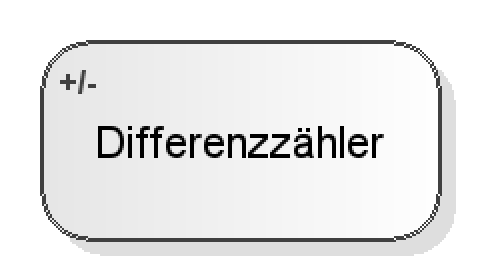
\includegraphics[width=2cm]{imageModelElementDifferentialCounter.png}
\vspace{-22pt}
\end{wrapfigure}

Durchläuft ein Kunde dieses Element, so wird der zugehörige Zähler um einen bestimmten Wert erhöht oder verringert.
Der Minimalwert des Zählers ist 0. Besitzen mehrere Differenzzähler denselben Namen, so wirken Sie auf dasselbe
Zähler-Objekt.

\subsection*{Einstellungen}

Der Name gibt das Zähler-Objekt an, welche jeweils beim Durchlauf eines Kunden durch das Element um den
angegebenen Wert verändert werden soll. Der Minimal- und zugleich auch Startwert eines jeden Zählers ist 0.


\section{Durchsatz}
\label{ref:ModelElementThroughput}

\begin{wrapfigure}{l}{2.5cm}
\vspace{-22pt}
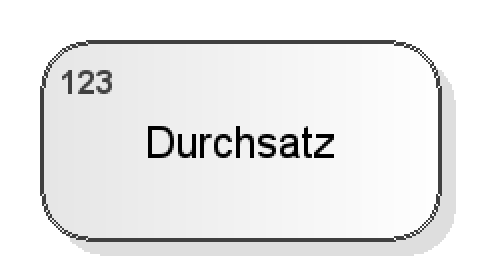
\includegraphics[width=2cm]{imageModelElementThroughput.png}
\vspace{-22pt}
\end{wrapfigure}

Durchläuft ein Kunde dieses Element, so wird der zugehörige Zähler um eins erhöht und gleichzeitig die
bislang verstrichene Zeit erfasst. Auf diese Weise kann erfasst werden,
wie viele Kunden jeweils pro Zeiteinheit durch das Element durchlaufen haben.

\subsection*{Einstellungen}

Der Name des Durchsatz-Elements hat besitzt keine weitere Bedeutung für die Simulations selbst.
Es muss jedoch ein Name angegeben werden, da der ermittelte Durchsatz unter diesem Namen in der
Statistik ausgewiesen wird.


\section{Kosten}
\label{ref:ModelElementCosts}

\begin{wrapfigure}{l}{2.5cm}
\vspace{-22pt}
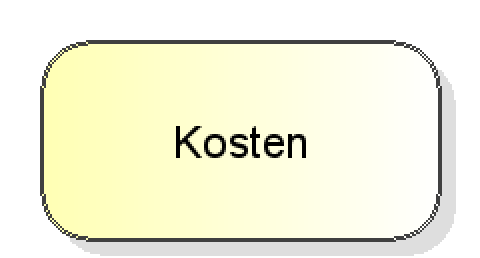
\includegraphics[width=2cm]{imageModelElementCosts.png}
\vspace{-22pt}
\end{wrapfigure}

Siehe auch Abschnitt \textbf{Sonstige Kosten} im Lehrbuch.

Passiert ein Kunde dieses Element, so werden optional Wartezeit-, Transferzeit- und/oder Bedienzeit-Kosten für ihn
verbucht. Außerdem können Kosten, die an der Station selber entstehen erfasst werden.

\subsection*{Einstellungen}

Der Name des Kosten-Elements hat keine weitere Bedeutung. Die angegebenen Kunden-Kosten werden in dem Kunden-Element,
das die Station passiert, erfasst. Des Weiteren können Kosten angegeben werden, die für die Station selber verbucht
werden.

Die optionale Bedingung ermöglicht es, dass nur unter bestimmten Voraussetzungen eine Zuweisung erfolgt,
wenn ein Kunde die Station passiert.


\section{Kundenstatistik}
\label{ref:ModelElementSetStatisticsMode}

\begin{wrapfigure}{l}{2.5cm}
\vspace{-22pt}
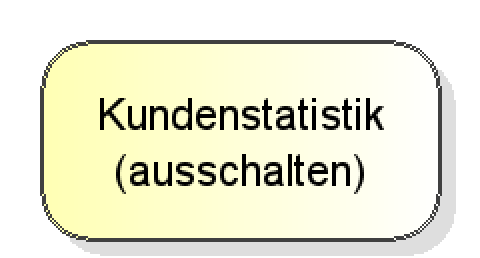
\includegraphics[width=2cm]{imageModelElementSetStatisticsMode.png}
\vspace{-22pt}
\end{wrapfigure}

Das Kundenstatistik-Element ermöglicht es, für die Kunden, die es passieren,
die Statistikerfassung ein oder aus zu schalten.

\subsection*{Einstellungen}

Der Name des Kundenstatistik-Elements hat keine weitere Bedeutung für die Simulation.
In den Einstellungen muss festgelegt werden, ob die Statistikerfassung für die Kunden,
die dieses Element passieren, ein oder ausgeschaltet werden soll.


\section{Multizähler}
\label{ref:ModelElementCounterMulti}

\begin{wrapfigure}{l}{2.5cm}
\vspace{-22pt}
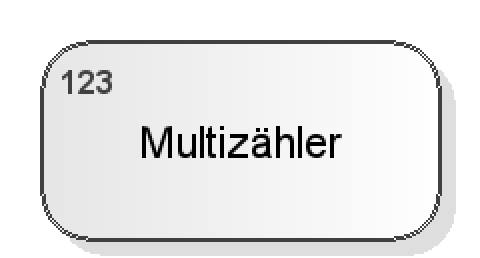
\includegraphics[width=2cm]{imageModelElementCounterMulti.png}
\vspace{-22pt}
\end{wrapfigure}

Durchläuft ein Kunde dieses Element, so wird in Abhängigkeit von verschiedenen Bedingungen
der Wert eines Zählers um eins erhöht. Auf diese Weise kann erfasst werden, wie viele Kunden
jeweils einen bestimmten Weg in dem Simulationsmodell gewählt haben. Ein Mehrfachzähler
entspricht einer Verzweigung (siehe Seite \pageref{ref:ModelElementDecide}) auf Basis von Bedingungen
gefolgt von jeweils normalen Zähler-Elementen (siehe Seite \pageref{ref:ModelElementCounter}) .

\subsection*{Einstellungen}

Der Name des Mehrfachzähler-Elements besitzt keine weitere Bedeutung für die Simulation.
Über einen Gruppennamen werden die Zähler in dem Elemente zu einer Gruppe zusammengefasst,
so dass in der Statistik neben dem Absolutwert der jeweiligen Zähler auch ein relativer
Wert angegeben werden kann. Passiert ein Kunde das Mehrfachzähler-Element, so werden die
angegebenen Bedingungen der Reihe nach geprüft. Bei der ersten erfüllten Bedingung wird
der entsprechende Zähler um eins erhöht. Ist keine der Bedingungen erfüllt, so wird der
für den ,,sonst''-Fall angegebene Zähler erhöht. 


\section{Script}
\label{ref:ModelElementSetJS}

\begin{wrapfigure}{l}{2.5cm}
\vspace{-22pt}
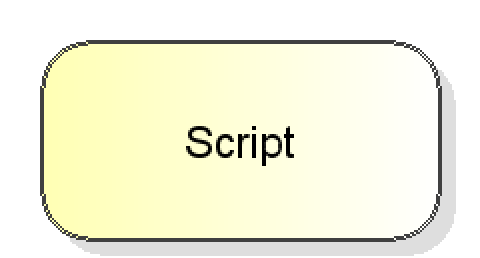
\includegraphics[width=2cm]{imageModelElementSetJS.png}
\vspace{-22pt}
\end{wrapfigure}

Durchläuft ein Kunde dieses Element, so wird das in ihm definierte Javascript- oder Java-Programm ausgeführt.

\subsection*{Einstellungen}

Der Name des Script-Elements hat keine weitere Bedeutung. Die auszuführenden Skriptbefehle werden in
\textbf{Javascript} oder in \textbf{Java} angegeben. Zusätzlich stehen einige
besondere Javascript-Befehle bzw. besondere Java-Befehle 
zum Zugriff auf die Simulationsdaten zur Verfügung.

\subsection*{Alternative}

Die Definition von Zuweisungen in Form eines Javascript- oder Java-Programms erlaubt eine größtmögliche Flexibilität,
benötigt jedoch verhältnismäßig viel Zeit. Eine schnellere Möglichkeit zur Zuweisung von Variablen
bietet das Variable-Element (siehe Seite \pageref{ref:ModelElementSet}) .


\section{Textzuweisung}
\label{ref:ModelElementAssignString}

\begin{wrapfigure}{l}{2.5cm}
\vspace{-22pt}
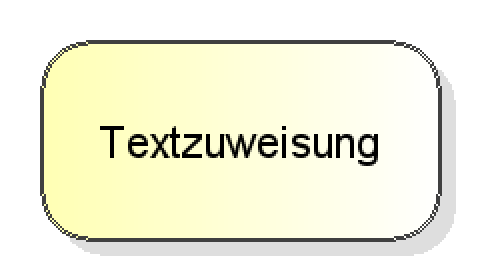
\includegraphics[width=2cm]{imageModelElementAssignString.png}
\vspace{-22pt}
\end{wrapfigure}

Das Textzuweisung-Element weist den Kunden, die es passieren, einen oder mehrere bestimmte Text
unter einem bestimmten Schlüsseln zu.

\subsection*{Einstellungen}

Der Name des Textzuweisung-Elements besitzt keine weitere Bedeutung für die Simulation. Bei jeder
Zuweisung muss ein nichtleerer Schlüssel angegeben werden. Als Werte können hingegen optional
leere Zeichenkette verwendet werden.

Die optionale Bedingung ermöglicht es, dass nur unter bestimmten Voraussetzungen eine Zuweisung erfolgt,
wenn ein Kunde die Station passiert.


\section{Typzuweisung}
\label{ref:ModelElementAssign}

\begin{wrapfigure}{l}{2.5cm}
\vspace{-22pt}
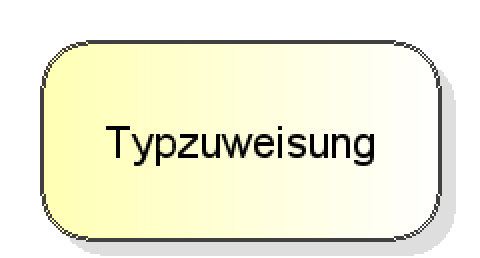
\includegraphics[width=2cm]{imageModelElementAssign.png}
\vspace{-22pt}
\end{wrapfigure}

Das Zuweisung-Element weist den Kunden, die es passieren, einen neuen Kundentyp dem sie in der Statistik zugeordnet werden sollen, zu.

\subsection*{Einstellungen}

Der Name des Zuweisungs-Elements ist gleichzeitig der Kundentyp, den alle Kunden, die dieses Element passieren, erhalten.

Die optionale Bedingung ermöglicht es, dass nur unter bestimmten Voraussetzungen eine Zuweisung erfolgt,
wenn ein Kunde die Station passiert.


\section{Variable}
\label{ref:ModelElementSet}

\begin{wrapfigure}{l}{2.5cm}
\vspace{-22pt}
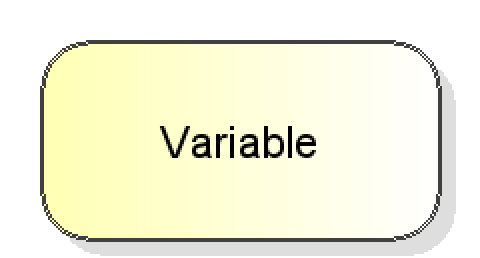
\includegraphics[width=2cm]{imageModelElementSet.png}
\vspace{-22pt}
\end{wrapfigure}

Durchläuft ein Kunde dieses Element, so werden die in ihm definierten Variablenzuweisungen durchgeführt.
In allen anderen Elementen, in denen Ausdrücke ausgewertet werden, allem voran in dem
Bedingung-Element (siehe Seite \pageref{ref:ModelElementHold}) , kann auf diese Variablen zugegriffen werden.

Initial werden alle neuen Variablen mit 0 belegt. Durch die Zuweisung \texttt{a:=a+1} lassen sich
Zähler realisieren.

\subsection*{Einstellungen}

Der Name des Variable-Elements hat keine weitere Bedeutung. Die Zuweisungen werden in der Reihenfolge, in der
sie in dem Element definiert sind, abgearbeitet, wenn ein Kunde das Element durchquert.

Über die drei Pseudo-Variablennamen ,,w'', ,,t'' und ,,p'' kann lesend und schreibend auf die Wartezeit, die Transferzeit
und die Bedienzeit des aktuellen Kunden (jeweils auf Sekundenbasis) zugegriffen werden. Außerdem kann statt eines
Variablennamens ein Kundenobjekt-Datenfeld über ,,ClientData(index)'' beschrieben werden.

Die optionale Bedingung ermöglicht es, dass nur unter bestimmten Voraussetzungen eine Zuweisung erfolgt,
wenn ein Kunde die Station passiert.

\subsection*{Alternative}

Mit dem Javascript-Element (siehe Seite \pageref{ref:ModelElementSetJS}) besteht die Möglichkeit, weit komplexere
Zuweisungen zu definieren. Allerdings benötigt der Simulator für die Ausführung
des Javascript-Elements deutlich mehr Rechenzeit.


\section{Zustand}
\label{ref:ModelElementStateStatistics}

\begin{wrapfigure}{l}{2.5cm}
\vspace{-22pt}
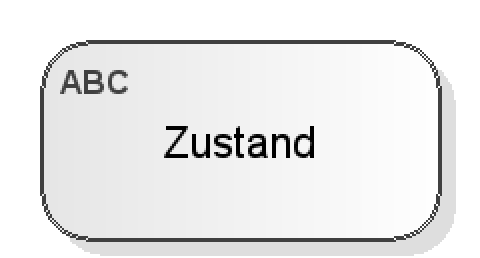
\includegraphics[width=2cm]{imageModelElementStateStatistics.png}
\vspace{-22pt}
\end{wrapfigure}

Durchläuft ein Kunde dieses Element, so wird der zugehörige Systemstatus in der Statistik gesetzt. 
Mit Hilfe von mehreren Zustandsstatistik-Elementen kann erfasst werden, wie lange sich das System
jeweils in einem bestimmten Zustand befunden hat.

\subsection*{Einstellungen}

Neben dem Namen muss noch ein Gruppenname für den Zustand angegeben werden. Neben dem jeweiligen
Absolutwert wird in der Statistik auch der Anteil der Zeit in dem Zustand brzogen auf die Gruppe ausgewiesen.


\section{Zähler}
\label{ref:ModelElementCounter}

\begin{wrapfigure}{l}{2.5cm}
\vspace{-22pt}
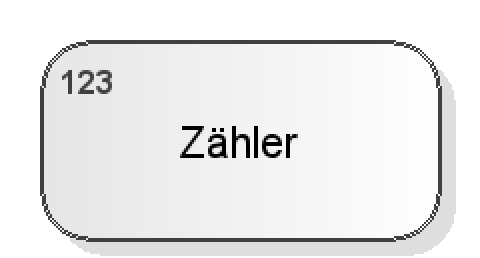
\includegraphics[width=2cm]{imageModelElementCounter.png}
\vspace{-22pt}
\end{wrapfigure}

Durchläuft ein Kunde dieses Element, so wird der zugehörige Zähler um eins erhöht. Auf diese Weise kann erfasst werden,
wie viele Kunden jeweils einen bestimmten Weg in dem Simulationsmodell gewählt haben.

\subsection*{Einstellungen}

Neben dem Namen muss noch ein Gruppenname für den Zähler angegeben werden. Neben dem jeweiligen
Absolutwert wird in der Statistik auch der Anteil des Zählers innerhalb seiner jeweiligen Gruppe ausgewiesen.





\chapter{Verzweigungen}

\section{Duplizieren}
\label{ref:ModelElementDuplicate}

\begin{wrapfigure}{l}{2.5cm}
\vspace{-22pt}
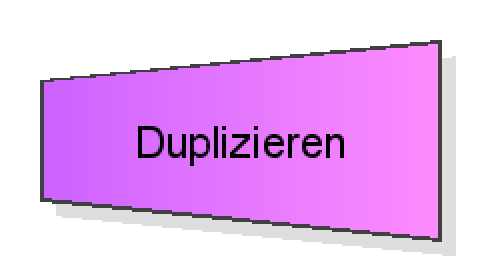
\includegraphics[width=2cm]{imageModelElementDuplicate.png}
\vspace{-22pt}
\end{wrapfigure}

In ein Duplizieren-Element können beliebig viele Kanten einlaufen. Alle Kunden, die über diese Kanten an dem Element eintreffen,
werden über die mehreren möglichen auslaufenden Kanten weitergeleitet. Laufen mehrere Kanten aus dem Element aus, so wird das
Kunden-Objekt dupliziert und es wird ein gleichartiges Objekt über jede der Kanten weitergeleitet.

\subsection*{Einstellungen}

Für das Duplizieren-Element kann ein Name eingestellt werden. Dieser hat jedoch keine weitere Bedeutung, sondern wird lediglich
in der Komponente auf der Zeichenfläche angezeigt. Des Weiteren können optionale Kundentypen für die auslaufenden Kanten angegeben
werden, die den Kunden, die das Element verlassen, zugewiesen werden.


\section{Verzweigen}
\label{ref:ModelElementDecide}

\begin{wrapfigure}{l}{2.5cm}
\vspace{-22pt}
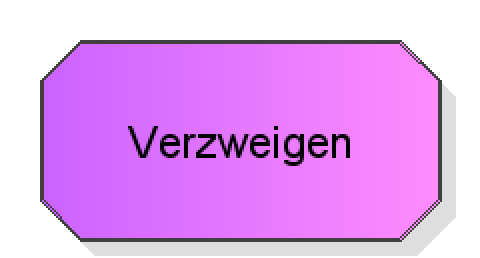
\includegraphics[width=2cm]{imageModelElementDecide.png}
\vspace{-22pt}
\end{wrapfigure}

Dieses Element ermöglicht es, die eintreffenden Kunden in mehrere mögliche Ausgangsrichtungen weiter zu leiten.
Die Verzweigung kann dabei nach folgenden Kriterien erfolgen:

\begin{itemize}
  \item 
    \textbf{Zufällig:}
    Pro Ausgangsrichtung wird eine Rate angegeben, die die Wahrscheinlichkeit für diesen Weg bestimmt.

  \item 
    \textbf{Bedingung:}
    Für alle Ausgangsrichtungen (außer für die letzte Richtung) wird eine Bedingung definiert. Trifft ein
    Kunde ein, so werden von oben nach unten diese Bedingungen geprüft. Der Kunde wird in die Richtung,
    bei der zum ersten Mal die Bedingung erfüllt war, weitergeleitet. Trifft keine der Bedingungen zu,
    so wird der Kunde in die letzte Richtung (für die keine Bedingung angegeben ist) weitergeleitet.    

  \item 
    \textbf{Kundentyp:}
    Für alle Ausgangsrichtungen (außer für die letzte Richtung) wird ein Kundentyp festgelegt. Ist ein
    eintreffender Kunde von einem dieser Typen, so wird er in die entsprechende Richtung weitergeleitet.
    Stimmt der Typ des eingetroffenen Kunden mit keinem der angegebenen Kundentypen überein,
    so wird der Kunde in die letzte Richtung (für die kein Kundentyp angegeben ist) weitergeleitet.

  \item 
    \textbf{Reihenfolge:}
    Es wird jeweils der Reihe nach einer der Kunden an einen der Ausgänge geleitet. Nachdem ein Kunde
    an den als letztes angebundenen Ausgang geleitet wurde, wird der nächste Kunde wieder an den
    ersten Ausgang geleitet. 

  \item 
    \textbf{Kürzeste Warteschlange an der nächsten Station:}
    Leitet den Kunden über den Pfad weiter, bei dem an der direkten Folgestation
    die Warteschlangenlänge minimal ist.

  \item 
    \textbf{Kürzeste Warteschlange an der nächsten Bedienstation:}
    Leitet den Kunden über den Pfad weiter, bei dem an der nächsten
    darin auftretenden Bedienstation die Warteschlangenlänge minimal ist.
    Andere Stationen, die zwischen dem Verzweigen-Element und der
    Bedienstation liegen, werden bei der Bestimmung der Warteschlangenlänge
    nicht berücksichtigt.

  \item 
    \textbf{Geringste Anzahl an Kunden an der nächsten Station:}
    Leitet den Kunden über den Pfad weiter, bei dem sich an der direkten Folgestation
    die geringste Anzahl an Kunden befinden.

  \item 
    \textbf{Geringste Anzahl an Kunden an der nächsten Bedienstation:}
    Leitet den Kunden über den Pfad weiter, bei dem sich an der nächsten
    darin auftretenden Bedienstation die geringste Anzahl an Kunden befinden.
    Andere Stationen, die zwischen dem Verzweigen-Element und der
    Bedienstation liegen, werden bei der Bestimmung der Anzahl an Kunden
    nicht berücksichtigt.

  \item 
    \textbf{Texteigenschaft:}
    Für alle Ausgangsrichtungen (außer für die letzte Richtung) wird ein Wert festgelegt.
    Wenn die Texteigenschaft des jeweiligen Kunden den jeweiligen Wert aufweist,
    so wird er in die entsprechende Richtung weitergeleitet.
    Stimmt der Wert mit keinem der angegebenen Wert überein,
    so wird der Kunde in die letzte Richtung (für die kein Wert angegeben ist) weitergeleitet.

\end{itemize}

\subsection*{Einstellungen}

\subsubsection*{Modus ,,Zufall''}

Die Weiterleitungswahrscheinlichkeiten in die verschiedenen möglichen Ausgangsrichtungen müssen nicht in
Form von Wahrscheinlichkeiten, die sich in ihrer Summe zu 1 aufaddieren müssen, angegeben werden, sondern
es genügt, Raten anzugeben. Diese Raten werden vom Programm automatisch zu Wahrscheinlichkeiten normiert.
Es gelten lediglich folgende Voraussetzungen: Die Raten dürfen nicht negativ sein und mindestens eine der
angegebenen Raten muss echt größer als 0 sein.

\subsubsection*{Modus ,,Bedingung''}

Pro vorhandener Verzweigung muss eine Bedingung angegeben werden, unter der die Kunden in diese Richtung
geleitet werden. Die Bedingungen müssen sich nicht gegenseitig ausschließen und werden von oben nach unten
abgearbeitet. Für die letzte Verzweigungsmöglichkeit kann keine Bedingung angegeben werden. Diese Verzweigung
wird in der Simulation immer dann gewählt, wenn keine der vorherigen Bedingungen zutreffend war.

\subsubsection*{Modus ,,Kundentyp''}

Pro vorhandener Verzweigung muss ein Kundentyp angegeben werden, dessen Kunden in diese Richtung
geleitet werden. Für die letzte Verzweigungsmöglichkeit kann kein Kundentyp angegeben werden. Diese Verzweigung
wird in der Simulation immer dann gewählt, wenn keine der vorherigen Bedingungen zutreffend war.

\subsubsection*{Modus ,,Texteigenschaft''}

Es muss ein Schlüssel, dessen Werte bei den Kunden betrachtet werden sollen, angegeben werden.
Außerdem muss pro vorhandener Verzweigung ein Wert angegeben werden. Kunden bei denen der Schlüssel
den angegebenen Wert besitzt, werden in diese Richtung geleitet. Für die letzte Verzweigungsmöglichkeit
kann kein Wert angegeben werden. Diese Verzweigung wird in der Simulation immer dann gewählt,
wenn keine der vorherigen Bedingungen zutreffend war.

Des Weiteren können in jedem Modus optionale Kundentypen für die auslaufenden Kanten angegeben
werden, die den Kunden, die das Element verlassen, zugewiesen werden.


\section{Verzweigen (Skript)}
\label{ref:ModelElementDecideJS}

\begin{wrapfigure}{l}{2.5cm}
\vspace{-22pt}
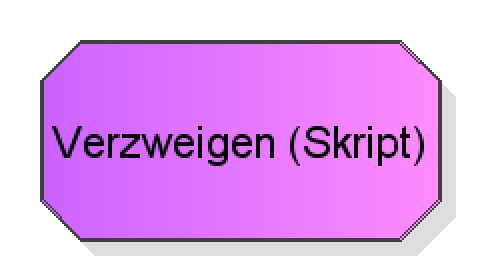
\includegraphics[width=2cm]{imageModelElementDecideJS.png}
\vspace{-22pt}
\end{wrapfigure}

Dieses Element ermöglicht es, die eintreffenden Kunden auf Basis von Javascript-Code
oder Java-Code in mehrere mögliche Ausgangsrichtungen weiter zu leiten.

\subsection*{Einstellungen}

Der Skript-Code kann beliebige Javascript-Befehle oder Java-Befehle enthalten
und kann über die zusätzlichen Javascript-Befehle bzw.
die zusätzlichen Java-Befehle auf das Simulationssystem
zugreifen. Als Rückgabewert (auszugeben über \texttt{Output.print()}) wird ein Zahlenwert
erwartet, der (1-basierend) die Nummer des zu wählenden Ausgangs angibt.


\section{Zurückschrecken}
\label{ref:ModelElementBalking}

\begin{wrapfigure}{l}{2.5cm}
\vspace{-22pt}
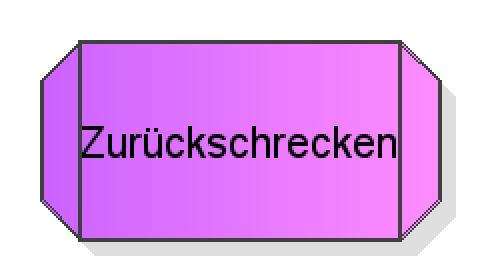
\includegraphics[width=2cm]{imageModelElementBalking.png}
\vspace{-22pt}
\end{wrapfigure}

Das Zurückschrecken-Element prüft, ob an der auf direktem Weg folgenden Bedienstation Kunden warten.
Wenn nein, wird der Kunde über den normalen Weg weitergeleitet.
Wenn ja, wird die Bedingung (die z.B. Zufallsausdrücke in Abhängigkeit von Kundeneigenschaften usw.
enthalten kann) ausgewertet. Trifft diese zu, so schreckt der Kunde davor zurück, sich an die
Warteschlange anzustellen und verlässt das Zurückschrecken-Element über den für diesen Fall
vorgesehenen zweiten Weg.

\subsection*{Einstellungen}

Der Name des Zurückschrecken-Elements hat keine weitere Bedeutung für die Simulation.
Der angegebene Ausdruck wird immer dann ausgewertet, wenn an der folgenden Bedienstation
eine Warteschlange vorhanden ist, und bestimmt, ob der Kunde bereit ist, sich anzustellen
oder ob er davor zurückschreckt. Als Ausdruck kann entweder eine Bedingung oder eine
Zurückschreckwahrscheinlichkeit angegeben werden. Die Angabe kann dabei global oder per
Kundentyp erfolgen.





\chapter{Schranken}

\section{Bedingung}
\label{ref:ModelElementHold}

\begin{wrapfigure}{l}{2.5cm}
\vspace{-22pt}
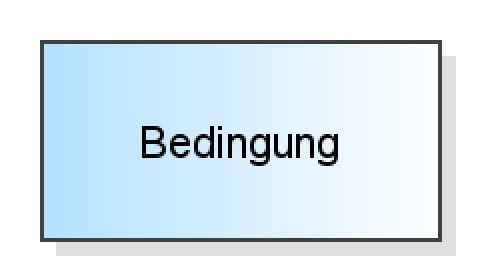
\includegraphics[width=2cm]{imageModelElementHold.png}
\vspace{-22pt}
\end{wrapfigure}

Siehe auch Abschnitte \textbf{Pull-Produktion im Warteschlangensimulator}

und \textbf{Verwendung der Simulationszeit} im Lehrbuch.

Bei dem Durchlaufen des Bedingung-Elements werden die Kunden so lange aufgehalten, bis die eingestellte Bedingung erfüllt ist. 

\subsection*{Einstellungen}

Der Name des Bedingung-Elements hat keine weitere Bedeutung. Befinden sich Kunden in der Warteschlange, so wird ständig geprüft,
ob die Bedingung erfüllt ist. Wenn ja, wird der Kunde mit der höchsten Priorität freigegeben. Danach wird eine (Simulationszeit) Millisekunde
gewartet bis die nächste Prüfung erfolgt und ggf. der nächste Kunde freigegeben wird. Es kann dabei eingestellt werden, ob die Bedingung global
betrachtet werden soll (ohne die Möglichkeit, kundenspezifische Variablen zu verwenden) oder ob die Bedingung kundenspezifisch interpretiert
werden soll (inkl. der Möglichkeit, kundenspezifische Variablen zu verwenden). Im Falle einer globalen Interpretation wird die Bedingung nur
einmal ausgewertet; wenn sie nicht zutrifft, wird die Verarbeitung in diesem Schritt abgeschlossen. Im Falle der kundenspezifischen Interpretation
wird die Bedingung in jedem Schritt für jeden wartenden Kunden einzeln ausgewertet (was die Simulation verlangsamt).
Gehen in die Bedingung Werte ein, die sich unabhängig von Ereignissen verändern können (z.B. die simulierte Zeit), so kann es notwendig sein,
die Option ,,Bedingung zusätzlich zeitgesteuert prüfen'' zu aktivieren. In diesem Fall wird der Wert der Bedingung zusätzlich in bestimmten
Zeitabständen geprüft. Wie lange diese Abstände sind, kann im Modelleigenschaften -Dialog konfiguriert
werden. Eine zusätzlich zeitabhängige Prüfung verlangsamt die Simulation signifikant und sollte nur aktiviert werden, wenn dies für die
jeweilige Bedingung zwingend erforderlich ist. 


\section{Bedingung (Skript)}
\label{ref:ModelElementHoldJS}

\begin{wrapfigure}{l}{2.5cm}
\vspace{-22pt}
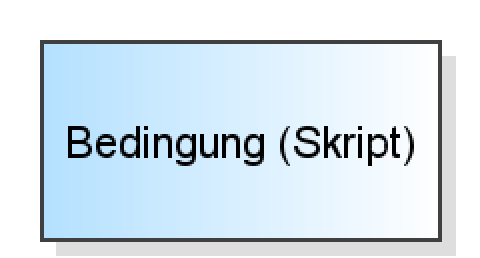
\includegraphics[width=2cm]{imageModelElementHoldJS.png}
\vspace{-22pt}
\end{wrapfigure}

Siehe auch Abschnitt \textbf{Pull-Produktion im Warteschlangensimulator} im Lehrbuch.

Dieses Element ermöglicht es, die eintreffenden Kunden auf Basis von Javascript-
oder Java-Code zu verzögern bzw. frei zu geben.

\subsection*{Einstellungen}

Der Skript-Code kann beliebige Javascript- und Java-Befehle enthalten und kann über
zusätzliche Javascript-Befehle bzw. zusätzlichen Java-Befehle 
auf das Simulationssystem zugreifen.

Gehen in die Bedingung Werte ein, die sich unabhängig von Ereignissen verändern können (z.B. die simulierte Zeit), so kann es notwendig sein,
die Option ,,Bedingung zusätzlich zeitgesteuert prüfen'' zu aktivieren. In diesem Fall wird der Wert der Bedingung zusätzlich in bestimmten
Zeitabständen geprüft. Wie lange diese Abstände sind, kann im Modelleigenschaften -Dialog konfiguriert
werden. Eine zusätzlich zeitabhängige Prüfung verlangsamt die Simulation signifikant und sollte nur aktiviert werden, wenn dies für die
jeweilige Bedingung zwingend erforderlich ist.

Since script executions are generally time-consuming, an additional condition can be specified.
Only if this condition is met the script will be executed. If no condition is defined, the script
is always be executed if clients are waiting at the station and the system state changes.


\section{Multibedingung}
\label{ref:ModelElementHoldMulti}

\begin{wrapfigure}{l}{2.5cm}
\vspace{-22pt}
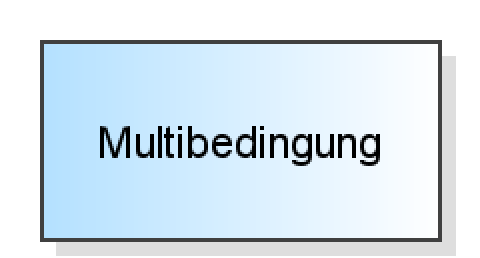
\includegraphics[width=2cm]{imageModelElementHoldMulti.png}
\vspace{-22pt}
\end{wrapfigure}

Siehe auch Abschnitt \textbf{Pull-Produktion im Warteschlangensimulator} im Lehrbuch.

Bei dem Durchlaufen des Mehrfachbedingung-Elements werden die Kunden so lange aufgehalten, bis eine der Bedingungen für eine
Ausgangskante erfüllt ist. Die Weiterleitung erfolgt dann in die Richtung, deren Bedingung erfüllt ist.

\subsection*{Einstellungen}

Der Name des Mehrfachbedingung-Elements hat keine weitere Bedeutung. Befinden sich Kunden in der Warteschlange, so wird ständig geprüft,
ob eine der Bedingungen erfüllt erfüllt ist. Wenn ja, wird der nächste Kunde freigegeben in die zu der erfüllten Bedingung
gehörigen Richtung freigegeben. Danach wird eine (Simulationszeit) Millisekunde gewartet bis die nächste
Prüfung erfolgt und ggf. der nächste Kunde freigegeben wird.
Gehen in die Bedingung Werte ein, die sich unabhängig von Ereignissen verändern können (z.B. die simulierte Zeit), so kann es notwendig sein,
die Option ,,Bedingung zusätzlich zeitgesteuert prüfen'' zu aktivieren. In diesem Fall wird der Wert der Bedingung zusätzlich in bestimmten
Zeitabständen geprüft. Wie lange diese Abstände sind, kann im Modelleigenschaften -Dialog konfiguriert
werden. Eine zusätzlich zeitabhängige Prüfung verlangsamt die Simulation signifikant und sollte nur aktiviert werden, wenn dies für die
jeweilige Bedingung zwingend erforderlich ist.


\section{Pull-Schranke}
\label{ref:ModelElementBarrierPull}

\begin{wrapfigure}{l}{2.5cm}
\vspace{-22pt}
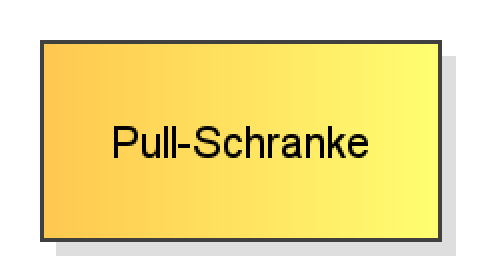
\includegraphics[width=2cm]{imageModelElementBarrierPull.png}
\vspace{-22pt}
\end{wrapfigure}

Siehe auch Abschnitt \textbf{Pull-Produktion im Warteschlangensimulator} im Lehrbuch.

Pull-Schranken ermöglichen es, die Anzahl an Kunden in einem bestimmten Segment
zu beschränken. Die Pull-Schranke lässt nur dann Kunden zur nächsten Station,
wenn die Gesamtzahl an Kunden beginnend von dieser Folgestation bis zu der angegebenen
nächsten (kontrollierten) Station einen Schwellenwert unterschreitet. Auf diese Weise
kann eine Pull-Wirkung durch die kontrollierte Station ausgeübt werden: Nur wenn an
dieser eine bestimmte Anzahl an Kunden unterschritten wird und in der aktuellen Station
auch nicht bereits genug Kunden vorhanden sind, um wieder auf die gewünschte Anzahl
zu kommen, werden weitere Kunden in die vordere Station gelassen.

\subsection*{Einstellungen}

Der Name des Pull-Schranke-Elements hat keine weitere Bedeutung. Es muss angegeben
werden, an welcher Station die Anzahl an Kunden kontrolliert werden soll und wie
viele Kunden sich dort maximal befinden dürfen.


\section{Ressource belegen}
\label{ref:ModelElementSeize}

\begin{wrapfigure}{l}{2.5cm}
\vspace{-22pt}
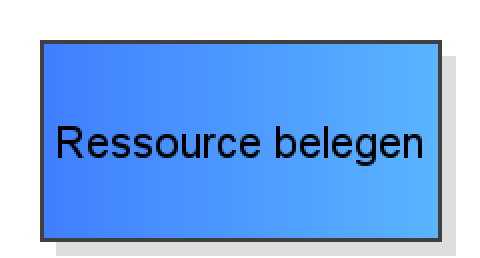
\includegraphics[width=2cm]{imageModelElementSeize.png}
\vspace{-22pt}
\end{wrapfigure}

Damit ein Kunde dieses Element passieren kann, müssen entsprechende Ressourcen verfügbar sein, die durch die Bewegung des
Kunden durch das Element belegt, aber nicht wieder freigegeben werden.

Die Freigabe muss später durch ein Ressourcen freigeben (siehe Seite \pageref{ref:ModelElementRelease}) Element erfolgen.

Die drei Elemente \textbf{Ressourcen belegen}, Verzögerung (siehe Seite \pageref{ref:ModelElementDelay}) und
Ressourcen freigeben (siehe Seite \pageref{ref:ModelElementRelease}) in dieser Reihenfolge arbeiten damit
insgesamt ähnlich wie ein Bedienstation (siehe Seite \pageref{ref:ModelElementProcess}) Element.

\subsection*{Einstellungen}

Für das Ressourcen belegen Elements muss ein Name angegeben werden, da sich die
Ressourcen freigeben (siehe Seite \pageref{ref:ModelElementRelease}) Elemente über die Namen
der Ressourcen belegen Elemente auf diese beziehen.

Um einen Kunden weiter zu leiten können mehrere Bediener aus mehreren Gruppen benötigt werden. Die Freigabe erfolgt
nur dann, wenn gleichzeitig alle notwendigen Bediener verfügbar werden und alle gleichzeitig belegt werden können.

Über die Ressourcen-Priorität kann festgelegt werden, mit welcher Priorität dieses Ressourcen belegen Element
berücksichtigt werden soll, wenn eine Ressource, die an dieser Station notwendig ist,
frei wird. Größere Werte bedeuten eine höhere Priorität bzw. eine höhere Wahrscheinlichkeit, dass dieses Element
die entsprechenden Ressourcen erhält, wenn es mehrere Stationen gibt, die dieselbe Ressource benötigen.

Zusätzlich kann eine maximale Wartezeit angegeben werden. Ist diese für einen Kunden verstrichen,
so verlässt er die Station über die zweite auslaufende Kante, ohne dass eine Ressourcenbelegung erfolgt.


\section{Ressource freigeben}
\label{ref:ModelElementRelease}

\begin{wrapfigure}{l}{2.5cm}
\vspace{-22pt}
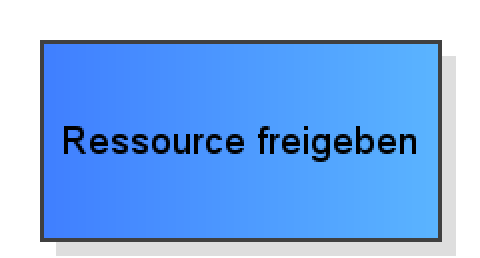
\includegraphics[width=2cm]{imageModelElementRelease.png}
\vspace{-22pt}
\end{wrapfigure}

In einem Ressourcen freigeben Element werden Ressourcen, die zuvor über ein Ressourcen belegen (siehe Seite \pageref{ref:ModelElementSeize}) 
Element belegt wurden, wieder freigegeben.

Die drei Elemente Ressourcen belegen (siehe Seite \pageref{ref:ModelElementSeize}) , Verzögerung (siehe Seite \pageref{ref:ModelElementDelay}) und
\textbf{Ressourcen freigeben} in dieser Reihenfolge arbeiten damit
insgesamt ähnlich wie ein Bedienstation (siehe Seite \pageref{ref:ModelElementProcess}) Element.

\subsection*{Einstellungen}

Der Name des Ressourcen freigeben Elements hat keine weitere Bedeutung. Es muss angegeben werden, mit welchem
Ressourcen belegen (siehe Seite \pageref{ref:ModelElementSeize}) Element dieses Element zusammenarbeiten soll.
Zusätzlich kann eine Zeitspanne angegeben werden, die zwischen der Ankunft eines Kunden an der Station und
der Freigabe der Ressourcen eingeplant werden soll. Ist eine solche Zeitspanne festgelegt, so hat der Kunde
das Freigabeelement bereits verlassen, wenn die zugehörigen Ressourcen tatsächlich freigegeben werden.  

\subsection*{Kundentypen laden}

Sollen an einer Station sehr viele Kundentypen mit unterschiedlichen Einstellungen verwendet werden, so können über diese Funktion mehrere Kundentypdaten aus einer Tabelle geladen werden. Jede Tabellenzeile enthält dabei die Daten zu einem Kundentyp.

Die erste Spalte muss den Namen des Kundentyps angeben, die zweite die Definition der entsprechenden Zeitdauer.
Dabei können die Zeitdauern entweder über einen Rechenausdruck oder über die Definition einer
Verteilungsfunktion festgelegt werden. Das Format der Verteilungsfunktionsdefinition ist in dem pdf-Dokument
"Distribution XML reference for Warteschlangensimulator'' dokumentiert.


\section{Schranke}
\label{ref:ModelElementBarrier}

\begin{wrapfigure}{l}{2.5cm}
\vspace{-22pt}
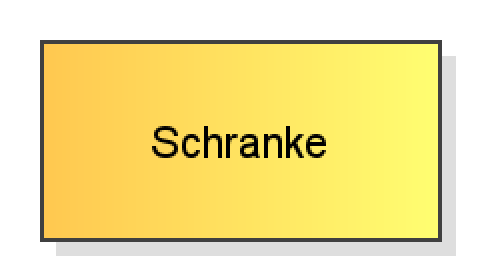
\includegraphics[width=2cm]{imageModelElementBarrier.png}
\vspace{-22pt}
\end{wrapfigure}

Siehe auch Abschnitt \textbf{Pull-Produktion im Warteschlangensimulator} im Lehrbuch.

An diesem Element werden eintreffende Kunden aufgehalten, bis ein Signal eintrifft, welches auf dessen Basis
eine Freigabe erfolgt. Entsprechende Signale werden durch Signal-Elemente (siehe Seite \pageref{ref:ModelElementSignal}) 
generiert, wenn sie von einem Kunden passiert werden.

\subsection*{Einstellungen}

Der Name des Schranke-Elements hat keine weitere Bedeutung. Es muss jedoch mindestens ein
Signal-Element (siehe Seite \pageref{ref:ModelElementSignal}) angegeben werden, welches die Freigabe
von hier wartenden Kunden signalisiert. Es kann dabei eingestellt werden,
wie viele wartende Kunden pro eintreffendem Signal maximal freigegeben werden sollen und ob sich
die Freigabe auf alle wartenden Kundentypen oder nur einen bestimmten Kundentyp beziehen soll.
Des Weiteren kann eine Anzahl an Kunden festgelegt werden, die die Schranke passieren dürfen,
bevor die Zählung beginnt. Trifft ein Signal ein, während kein Kunde wartet, so kann angegeben
werden, ob dies für einen später dann sofort freizugebenden Kunden gespeichert werden soll,
oder ob es verworfen werden soll.


\section{Signal}
\label{ref:ModelElementSignal}

\begin{wrapfigure}{l}{2.5cm}
\vspace{-22pt}
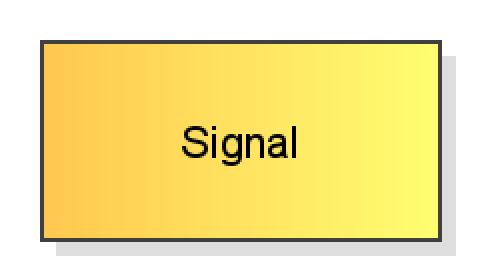
\includegraphics[width=2cm]{imageModelElementSignal.png}
\vspace{-22pt}
\end{wrapfigure}

Siehe auch Abschnitt \textbf{Pull-Produktion im Warteschlangensimulator} im Lehrbuch.

Passiert ein Kunde ein Signal-Element, so wird das Signal, welches dem Namen des Elements entspricht, ausgelöst.
Schranken-Elemente (siehe Seite \pageref{ref:ModelElementBarrier}) können durch solch ein Signal benachrichtigt werden und
wartende Kunden freigeben.

\subsection*{Einstellungen}

Der Name des Signal-Elements ist gleichzeitig der Name des Signal, das ausgelöst wird, wenn ein Kunde das Element passiert.
Zusätzlich kann eine Zeitdauer eingestellt werden, um die die Auslösung des Signals nach dem Eintreffen des Kunden verzögert werden soll.
Ist keine Verzögerungszeit eingestellt, so wird das Ereignis ausgelöst, sobald ein Kunde an der Station eintrifft.





\chapter{Kunden verbinden}

\section{Ausleiten}
\label{ref:ModelElementPickUp}

\begin{wrapfigure}{l}{2.5cm}
\vspace{-22pt}
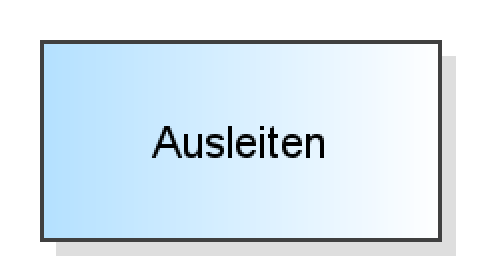
\includegraphics[width=2cm]{imageModelElementPickUp.png}
\vspace{-22pt}
\end{wrapfigure}

Siehe auch Abschnitt \textbf{Ausleiten-Stationen} im Lehrbuch.

Passiert ein Kunde dieses Element, so wird aus der Warteschlange eines anderen Elements ebenfalls ein Kunde entnommen
und gemeinsam mit dem aktuellen Kunden auf dem neuen Weg weitergeleitet oder wird mit dem aktuellen Kunden
zu einen temporären oder dauerhaften Batch zusammengefasst.

\subsection*{Einstellungen}

Der Name des Ausleiten-Elements hat keine weitere Bedeutung. Über die Angabe eines 
Bedienstation (siehe Seite \pageref{ref:ModelElementProcess}) -, Bedingung (siehe Seite \pageref{ref:ModelElementHold}) -
oder Schranke-Element (siehe Seite \pageref{ref:ModelElementBarrier}) s kann angegeben werden, aus welcher Warteschlange
der Kunde, der gemeinsam mit dem aktuellen Kunden weitergeleitet werden soll, bezogen werden soll.
Es kann angegeben werden, ob der aktuelle Kunde, wenn sich in der Warteschlange des anderen Elements kein
Kunde befindet, alleine weitergeleitet werden soll, oder ob solange gewartet werden soll, bis in der
anderen Warteschlange ein Kunde vorhanden ist. Des Weiteren kann eingestellt werden,
ob die zusammengeführten Kunden die Station einfach wieder (zeitlich gemeinsam) verlassen, ob die Kunden zu einem temporären
Batch zusammengefasst werden sollen (der später über das Batch auflösen (siehe Seite \pageref{ref:ModelElementSeparate}) Element
wieder aufgelöst werden kann) oder ob für die Kunden der Weg durch
das Netz an dieser Stelle endet (weil die beiden Kunden z.B. Teilkomponenten darstellen, die zu einem größeren Element
zusammengesetzt werden) und statt dessen ein neues Kundenobjekt erzeugt und ab diesem Punkt gestartet wird. 


\section{Multizusammenfassen}
\label{ref:ModelElementBatchMulti}

\begin{wrapfigure}{l}{2.5cm}
\vspace{-22pt}
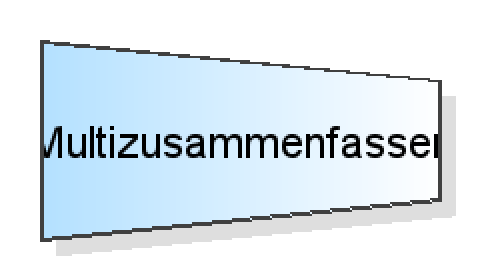
\includegraphics[width=2cm]{imageModelElementBatchMulti.png}
\vspace{-22pt}
\end{wrapfigure}

Siehe auch Abschnitt \textbf{Temporäre und permanente Batch-Bildung} im Lehrbuch.

In diesem Element müssen eintreffende Kunden warten, bis eine bestimmte Anzahl an Kunden vorhanden ist.
Diese werden dann gleichzeitig weitergeleitet oder zu einen temporären oder dauerhaften Batch zusammengefasst.
Im Unterschied zu der Zusammenfassen (siehe Seite \pageref{ref:ModelElementBatch}) -Station kann an dieser Station
pro Kundentyp konfiguriert werden, wie viele Kunden jeweils auf welche Weise zusammengefasst werden sollen.

\subsection*{Einstellungen}

Der Name des Zusammenfassen-Elements hat keine weitere Bedeutung. Über die minimale und die maximale Batch-Größe kann
eingestellt werden, wie viele Kunden in dem Zusammenfassen-Element minimal eingetroffen sein müssen, damit diese 
weitergeleitet werden bzw. wie viele maximal in einen Batch aufgenommen werden. Des Weiteren kann eingestellt werden,
ob die zusammengeführten Kunden die Station einfach wieder (zeitlich gemeinsam) verlassen, ob die Kunden zu einem temporären
Batch zusammengefasst werden sollen (der später über das Batch auflösen (siehe Seite \pageref{ref:ModelElementSeparate}) Element
wieder aufgelöst werden kann) oder ob für die Kunden der Weg durch
das Netz an dieser Stelle endet (weil die beiden Kunden z.B. Teilkomponenten darstellen, die zu einem größeren Element
zusammengesetzt werden) und statt dessen ein neues Kundenobjekt erzeugt und ab diesem Punkt gestartet wird.
Kunden, für deren Typ keine Batch-Bildungsregel definiert ist, passieren die Station ohne weitere Verzögerung.

Werden die eintreffenden Kunden zu einem temporären oder einem permanenten Batch verbunden, so kann eingestellt werden
ob und wenn ja auf welche Weise die Zeitdauern (Wartezeit, Bedienzeit, ...) sowie die nutzerdefinierten Datenfelder
der Einzelkunden auf das Batch-Objekt übertragen werden sollen.

\subsection*{Hinweis zu den Batch-Größen}

Batch-Größen müssen positive Ganzzahlen sein.
Es können auch Rechenausdrücke für die Batch-Größen angegeben werden.
Wenn diese Variablen oder Funktionen enthalten, die erst im Simulationskontext gültig sind, so werden diese zu Beginn der Simulation \textbf{einmalig} ausgewertet.
Das bedeutet, dass sich die an einer Station eingestellten Batch-Größen während einer laufenden Simulation nicht verändern.


\section{Trennen}
\label{ref:ModelElementSeparate}

\begin{wrapfigure}{l}{2.5cm}
\vspace{-22pt}
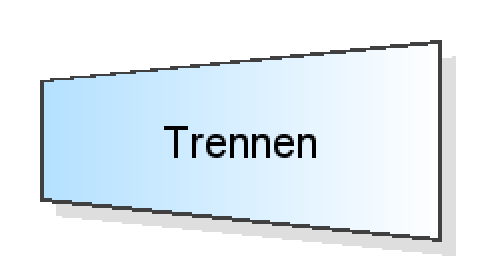
\includegraphics[width=2cm]{imageModelElementSeparate.png}
\vspace{-22pt}
\end{wrapfigure}

Siehe auch Abschnitt \textbf{Temporäre und permanente Batch-Bildung} im Lehrbuch.

Bewegt sich ein Batch durch dieses Element, so wird der Batch in die einzelnen Kunden, aus denen er
besteht, aufgelöst. Entsprechende Batches können in den Elementen Zusammenfassen (siehe Seite \pageref{ref:ModelElementBatch}) ,
Zusammenführen (siehe Seite \pageref{ref:ModelElementMatch}) und Ausleiten (siehe Seite \pageref{ref:ModelElementPickUp}) 
gebildet werden.

\subsection*{Einstellungen}

Der Name des Batch auflösen Elements hat keine weitere Bedeutung.


\section{Zerteilen}
\label{ref:ModelElementSplit}

\begin{wrapfigure}{l}{2.5cm}
\vspace{-22pt}
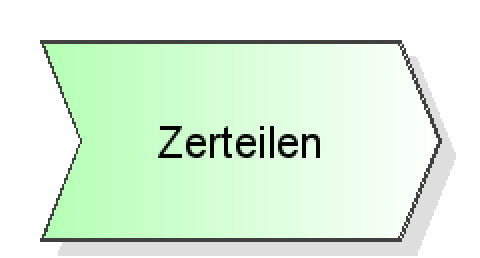
\includegraphics[width=2cm]{imageModelElementSplit.png}
\vspace{-22pt}
\end{wrapfigure}

Siehe auch Abschnitt \textbf{Zerteilen-Stationen} im Lehrbuch.

Trifft ein Kunde an einer Zerteilen-Station ein, so endet an dieser sein
Lebenszyklus vergleichbar einem Ausgang-Element (siehe Seite \pageref{ref:ModelElementDispose}) .
Dafür werden an der Station einer oder mehrere neue Kunden generiert, vergleichbar
einer Mehrfachquelle (siehe Seite \pageref{ref:ModelElementSourceMulti}) .

\subsection*{Einstellungen}

Der Name des Zerteilen-Elements besitzt keine weitere Bedeutung für die Simulation.

Pro Kunden-Teilquelle können folgende Eigenschaften eingestellt werden: 

Zunächst muss ein \textbf{Name} für den Typ der zu generierenden Kunden angegeben werden.
Der Dialog besitzt eine Reihe von Registerkarten, über die die verschiedenen Eigenschaften
der Kundenquelle konfiguriert werden können:

\subsubsection*{Batch-Größe}

Über die Batch-Größe kann zusätzlich
angegeben werden, dass pro Ankunft nicht ein einzelner Kunde, sondern zeitgleich jeweils
mehrere Kunden eintreffen sollen. Dabei kann eingestellt werden, dass immer gleich
viele Kunden pro Ankunft eintreffen (fest Batch-Größe) oder aber es kann eine Verteilung
der Raten, gemäß denen die jeweilige Größe des Ankunfts-Batches bestimmt werden soll,
angegeben werden.

\subsubsection*{Zuweisung von Kundenvariablen}

Auf dieser Registerkarte können Kundenvariablen vom Typ \texttt{ClientData(nr)} eingetragen werden,
die jedem neu erstellten Kunden automatisch zugewiesen werden sollen.

\subsubsection*{Zuweisung von Texten}

Auf dieser Registerkarte können Textzuweisungen vom Typ Schlüssel:=Text eingetragen werden,
die jedem neu erstellten Kunden automatisch zugewiesen werden sollen.

\subsubsection*{Übertragung der Kundendaten vom Ausgangskunden}

Unabhängig von den Einstellungen pro Teil-Kundenquelle kann eingestellt werden,
dass die numerischen und Text-basierenden Kundendaten von dem Ausgangskunden
auf die neu generierten Kunden übertragen werden sollen.

\subsection*{Kundentypen laden}

Sollen in einem Modell sehr viele Kundentypen verwendet werden, so können über diese Funktion Funktion mehrere
Kundentypen aus einer Tabelle geladen werden. Jede Tabellenzeile enthält dabei die Daten zu einem Kundentyp.

Die erste Spalte muss den Namen des Kundentyps angeben, die zweite die Definition der Zwischenankunftszeiten.
Dabei können die Zwischenankunftszeiten entweder über einen Rechenausdruck oder über die Definition einer
Verteilungsfunktion festgelegt werden. Das Format der Verteilungsfunktionsdefinition ist in dem pdf-Dokument
"Distribution XML reference for Warteschlangensimulator'' dokumentiert. Auf diese beiden Spalten können beliebig
viele weitere Spalten mit folgenden Inhalten folgen:

\begin{itemize}
  \item \texttt{batch=}<br>
  Gibt die Ankunfts-Batch-Größe an. Es kann entweder eine positive Ganzzahl angegeben werden oder eine Reihe von
  durch ,,;'' getrennte Werte der Form \texttt{Größe=Rate} zur Definition verschiedener Raten für verschiedene Batch-Größen. 
\end{itemize}

Außerdem stehen die Zuweisungen, die an einer Tabellenquelle (siehe Seite \pageref{ref:ModelElementSourceTable}) genutzt werden können, zur Verfügung.


\section{Zusammenfassen}
\label{ref:ModelElementBatch}

\begin{wrapfigure}{l}{2.5cm}
\vspace{-22pt}
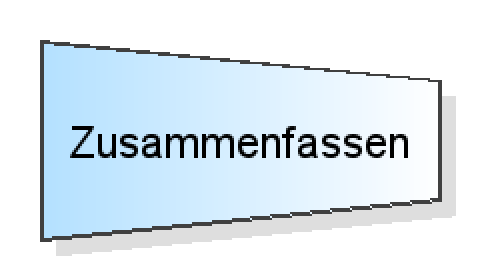
\includegraphics[width=2cm]{imageModelElementBatch.png}
\vspace{-22pt}
\end{wrapfigure}

Siehe auch Abschnitt \textbf{Temporäre und permanente Batch-Bildung} im Lehrbuch.

In diesem Element müssen eintreffende Kunden warten, bis eine bestimmte Anzahl an Kunden vorhanden ist.
Diese werden dann gleichzeitig weitergeleitet oder zu einen temporären oder dauerhaften Batch zusammengefasst.

\subsection*{Einstellungen}

Der Name des Zusammenfassen-Elements hat keine weitere Bedeutung. Über die minimale und die maximale Batch-Größe kann
eingestellt werden, wie viele Kunden in dem Zusammenfassen-Element minimal eingetroffen sein müssen, damit diese 
weitergeleitet werden bzw. wie viele maximal in einen Batch aufgenommen werden. Des Weiteren kann eingestellt werden,
ob die zusammengeführten Kunden die Station einfach wieder (zeitlich gemeinsam) verlassen, ob die Kunden zu einem temporären
Batch zusammengefasst werden sollen (der später über das Batch auflösen (siehe Seite \pageref{ref:ModelElementSeparate}) Element
wieder aufgelöst werden kann) oder ob für die Kunden der Weg durch
das Netz an dieser Stelle endet (weil die beiden Kunden z.B. Teilkomponenten darstellen, die zu einem größeren Element
zusammengesetzt werden) und statt dessen ein neues Kundenobjekt erzeugt und ab diesem Punkt gestartet wird.

Werden die eintreffenden Kunden zu einem temporären oder einem permanenten Batch verbunden, so kann eingestellt werden
ob und wenn ja auf welche Weise die Zeitdauern (Wartezeit, Bedienzeit, ...) sowie die nutzerdefinierten Datenfelder
der Einzelkunden auf das Batch-Objekt übertragen werden sollen.

\subsection*{Hinweis zu den Batch-Größen}

Batch-Größen müssen positive Ganzzahlen sein.
Es können auch Rechenausdrücke für die Batch-Größen angegeben werden.
Wenn diese Variablen oder Funktionen enthalten, die erst im Simulationskontext gültig sind, so werden diese zu Beginn der Simulation \textbf{einmalig} ausgewertet.
Das bedeutet, dass sich die an einer Station eingestellten Batch-Größen während einer laufenden Simulation nicht verändern.


\section{Zusammenführen}
\label{ref:ModelElementMatch}

\begin{wrapfigure}{l}{2.5cm}
\vspace{-22pt}
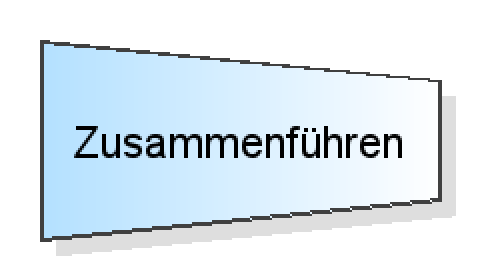
\includegraphics[width=2cm]{imageModelElementMatch.png}
\vspace{-22pt}
\end{wrapfigure}

Siehe auch Abschnitt \textbf{Zusammenführen-Stationen} im Lehrbuch.

Das Zusammenführen-Element besitzt zwei oder mehr Eingänge. Wenn an jedem der Eingänge ein Kunde vorhanden ist,
werden diese zeitgleich gemeinsam weitergeleitet oder zu einen temporären oder dauerhaften Batch zusammengefasst.
Sind nur an einem Eingang Kunden vorhanden, so müssen diese warten, bis auch an den anderen Eingängen Kunden eingetroffen sind.
Zusätzlich kann als Einschränkung eingestellt werden, dass nur Kunden zusammengeführt werden, bei denen ein bestimmtes
Kundendatenfeld denselben Zahlen- oder Textwert aufweist und es kann eine optionale Bedingung definiert werden,
die für das Zusammenführen erfüllt sein muss.

\subsection*{Einstellungen}

Der Name des Zusammenführen-Elements hat keine weitere Bedeutung. Es kann eingestellt werden, ob die zusammengeführten
Kunden die Station einfach wieder (zeitlich gemeinsam) verlassen, ob die Kunden zu einem temporären
Batch zusammengefasst werden sollen (der später über das Batch auflösen (siehe Seite \pageref{ref:ModelElementSeparate}) Element
wieder aufgelöst werden kann) oder ob für die Kunden der Weg durch das Netz an
dieser Stelle endet (weil die beiden Kunden z.B. Teilkomponenten darstellen, die zu einem größeren Element zusammengesetzt
werden) und statt dessen ein neues Kundenobjekt erzeugt und ab diesem Punkt gestartet wird.
Außerdem kann optional ein Kundendatenfeld angegeben werden, welches beim Abgleich der Kunden berücksichtigt werden soll,
so dass Kunden nur dann gemeinsam weitergeleitet werden, wenn für sie der Wert dieses Feldes identisch ist und es kann
optional eine Bedingung, die erfüllt sein muss, wenn Kundenobjekte zusammengeführt werden sollen.

Werden die eintreffenden Kunden zu einem temporären oder einem permanenten Batch verbunden, so kann eingestellt werden
ob und wenn ja auf welche Weise die Zeitdauern (Wartezeit, Bedienzeit, ...) sowie die nutzerdefinierten Datenfelder
der Einzelkunden auf das Batch-Objekt übertragen werden sollen.





\chapter{Transport}

\section{Duplizieren und Teleportieren}
\label{ref:ModelElementTeleportSourceMulti}

\begin{wrapfigure}{l}{2.5cm}
\vspace{-22pt}
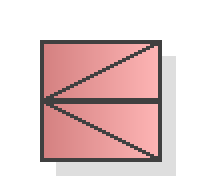
\includegraphics[width=2cm]{imageModelElementTeleportSourceMulti.png}
\vspace{-22pt}
\end{wrapfigure}

Teleport-Transporte ermöglichen es, einen Kunden ohne Zeitverzug
von einem Teleport-Transport Startpunkt zu einem 
Teleport-Transport Zielpunkt (siehe Seite \pageref{ref:ModelElementTeleportDestination}) 
zu bewegen. Im Gegensatz zu normalen Transporten geht es hierbei nicht darum,
einen tatsächlichen Transport eines Kunden (der eine gewisse Zeit dauern und
Ressourcen benötigen kann) zu modellieren, sondern darum dass Modell übersichtlich
zu halten. Betritt ein Kunde einen Teleport-Transport Startpunkt, so wird er
augenblicklich zu dem dort angegeben Teleport-Transport Zielpunkt befördert.
Start- und Zielpunkt können sich an verschiedenen Stellen im Modell befinden;
im Gegensatz zu einem Transport über eine Kante wird keine Verbindunglinie
zwischen Start und Ziel eingezeichnet.

Eine Duplizieren und Teleportieren Station kombiniert die Funktionalität
einer Duplizieren (siehe Seite \pageref{ref:ModelElementDuplicate}) -Station mit einer
Teleport-Transport Startpunkt (siehe Seite \pageref{ref:ModelElementTeleportSource}) -Station:
Zunächst wird das Kundenobjekt in mehrere gleichartige Objekte (mit stets denselben Daten)
aufgeteilt. Dann werden die Kundenobjekte zu allen in der Station konfigurierten Zielen
gleichzeitig geschickt.

\subsection*{Einstellungen}

Der Name des Duplizieren und Teleportieren Station besitzt keine weitere Bedeutung
für die Simulation. Allerdings müssen Name der
Teleport-Transport Zielpunkt (siehe Seite \pageref{ref:ModelElementTeleportDestination}) 
Elements angegeben werden, zu denen die eintreffenden Kunden befördert werden sollen.
Die Liste der Namen der Ziele gibt dabei auch gleichzeitig an, wie viele Kopien
des Kundenobjektes erzeugt werden sollen. Es können einzelne Ziele auch mehrfach
ausgewählt werden; in diesem Fall werden mehrere Kundenobjekte zu dem jeweiligen Ziel geschickt.  


\section{Fließband}
\label{ref:ModelElementConveyor}

\begin{wrapfigure}{l}{2.5cm}
\vspace{-22pt}
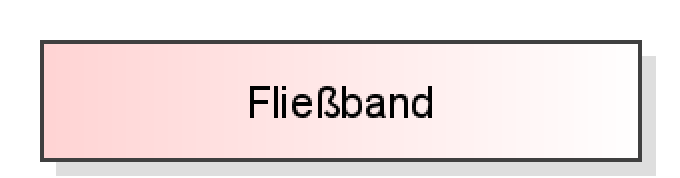
\includegraphics[width=2cm]{imageModelElementConveyor.png}
\vspace{-22pt}
\end{wrapfigure}

Siehe auch Abschnitt \textbf{Fließbandtransporte} im Lehrbuch.

Ein Fließband stellt eine feste Verzögerung für alle eintreffenden Kunden dar.
Zusätzlich besitzt ein Fließband eine begrenzte Kapazität und jeder Kunde
kann verschieden viel dieser Kapazität benötigen. So lange nicht genug
Kapazität verfügbar ist, um bestimmte Kunden zu transportieren, müssen diese
in einer Warteschlange warten.

\subsection*{Einstellungen}

Der Name des Fließband-Elements besitzt keine weitere Bedeutung
für die Simulation. Für ein Fließband kann eingestellt werden,
wie viele Kapazität dieses besitzt und wie viel Kapazität ein
Kunde benötigt (optional differenzierbar nach Kundentypen). Der
Transport der Kunden über das Fließband nimmt eine feste Zeit in
Anspruch, d.h. ein Kunde kann keinen anderen Kunden überholen.
Außerdem kann für die Animation eingestellt werden, ob sich die
Kunden in der Darstellung von links nach rechts oder von rechts
nach links bewegen sollen.


\section{Haltestelle}
\label{ref:ModelElementTransportTransporterSource}

\begin{wrapfigure}{l}{2.5cm}
\vspace{-22pt}
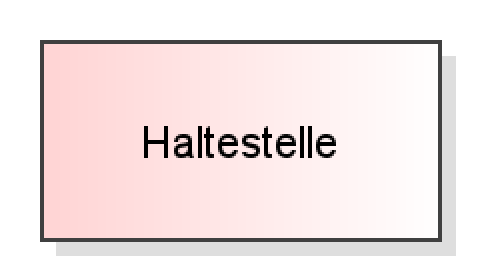
\includegraphics[width=2cm]{imageModelElementTransportTransporterSource.png}
\vspace{-22pt}
\end{wrapfigure}

Siehe auch Abschnitt \textbf{Transporte mit Transportern} im Lehrbuch.

Ein Haltestelle-Element ermöglicht den Transport eines Kunden zu einem beliebigen
Transportziel-Element (siehe Seite \pageref{ref:ModelElementTransportDestination}) . Wie viel
Zeit der Transport beansprucht und zu welchem Zielelement der Kunde transportiert
wird, kann dabei in dem Haltestelle-Element eingestellt werden.
Für den Transport eines Kunden von einem Transportstart- zu einem Transportzielelement
muss keine Verbindungskante zwischen den Elementen bestehen.
Im Gegensatz zu dem Transportstart-Element (siehe Seite \pageref{ref:ModelElementTransportSource}) 
werden im Haltestelle-Element keine Ressourcen (die keinen bestimmten Ort besitzen),
sondern Transporter, die sich zwischen den Stationen bewegen, verwendet.

\subsection*{Einstellungen}

Der Name des Haltestellen-Elements besitzt keine weitere Bedeutung.

Auf der Dialogseite \textbf{Transporter} kann festgelegt werden, welchen
Typ der Transporter zum abholen der wartenden Kunden besitzen muss,
wie viele Kunden warten müssen, bevor ein Transporter angefordert wird
und welche Priorität das Haltenstellen-Element in Bezug auf die
Anforderung von Transportern besitzen soll.
Des Weiteren können auch ohne wartende Kunden Transporter angefordert
werden, die dann in dem Element parken. Auch hierfür kann eine Priorität
und eine maximale Kapazität angegeben werden.

Auf der Dialogseite \textbf{Transportziele} können ein oder mehrere
mögliche Ziel für den Transport des Kunden angegeben werden. Für die Ziele können dabei
Bedingungen oder Kundentypen angegeben werden. Alternativ kann eingestellt werden, dass
das anzusteuernde Ziel aus dem Fertigungsplan des Kunden oder aus einer Texteigenschaft
des Kunden entnommen werden soll.

Auf der Dialogseite \textbf{Prioritäten} kann angegeben werden, welche
Kunden mit welcher Priorität einen Platz in einem eintreffenden
Transporter erhalten sollen.
Die Variable ,,w'' gibt dabei abweichend von der sonst üblichen Belegung die bisherige
Wartezeit des Kunden an der aktuellen Station an (und nicht die gesamte bisherige
Wartezeit des Kunden).

Auf der Dialogseite \textbf{Bereich verlassen} kann optional eine
Bereich-betreten-Station angegeben werden. Beim Start des Transports
wird dann der angegebene Bereich verlassen.


\section{Parkplatz}
\label{ref:ModelElementTransportParking}

\begin{wrapfigure}{l}{2.5cm}
\vspace{-22pt}
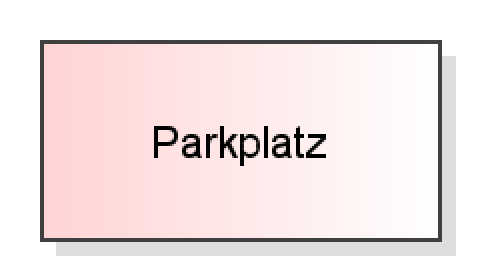
\includegraphics[width=2cm]{imageModelElementTransportParking.png}
\vspace{-22pt}
\end{wrapfigure}

Siehe auch Abschnitt \textbf{Transporte mit Transportern} im Lehrbuch.

Gibt es keine Station, die einen Transporter nach dem er sein Ziel erreicht hat
anfordert, so verbleibt der Transporter zunächst an der Zielstation. Wird er später
von einer Quellstation angefordert, so muss er ggf. einen weiten Weg zu ihr zurücklegen.
Ein Parkplatz-Element kann Transporter genauso wie eine Quellstation anfordern.
Allerdings erfolgt auf einem Parkplatz keine Beladung des Transporters, sondern er
bleibt hier einfach stehen. Der Vorteil besteht darin, dass ein Parkplatz deutlich
näher an einer Quellstation angeordent sein kann, so dass keine lange Anfahrtzeit
notwendig ist, wenn der Transporter benötigt wird.

\subsection*{Einstellungen}

Der Name des Parkplatzelements besitzt keine weitere Bedeutung.
Über das \textbf{Transportertyp}-Auswahlfeld kann festgelegt werden, welchen
Transportertyp dieser Parkplatz jeweils anziehen soll. Die \textbf{Parkplatzkapazität}
gibt an, wie viele Transporter maximal auf dem Parkplatz stehen können.
Die \textbf{Priorität zum Anfordern freier Transporter} sollte stets niedriger
gewählt sein, als die Priorität zum Anfordern freier Transporter von Quellstationen.
Andernfalls steuert einer freier Transporter eher einen Parkplatz an als eine
Station an der er benötigt wird.


\section{Plan zuweisen}
\label{ref:ModelElementAssignSequence}

\begin{wrapfigure}{l}{2.5cm}
\vspace{-22pt}
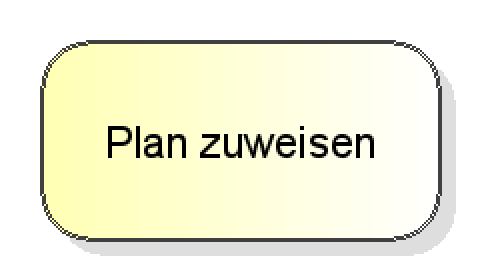
\includegraphics[width=2cm]{imageModelElementAssignSequence.png}
\vspace{-22pt}
\end{wrapfigure}

Siehe auch Abschnitt \textbf{Fertigungspläne} im Lehrbuch.

Das Fertigungsplan-Zuweisungs-Element weist den Kunden, die es passieren, einen Fertigungsplan zu.
Der Fertigungsplan kommt in den Transportstart (siehe Seite \pageref{ref:ModelElementTransportSource}) 
Elementen zur Bestimmung des Transportziels zum Tragen.

\subsection*{Einstellungen}

Der Name des Fertigungsplan-Zuweisungs-Elements hat keine weitere Bedeutung. Allerdings muss ein Fertigungsplan
ausgewählt werden, der den Kunden, die dieses Element passieren, zugewiesen werden soll.


\section{Teleport-Transport Startpunkt}
\label{ref:ModelElementTeleportSource}

\begin{wrapfigure}{l}{2.5cm}
\vspace{-22pt}
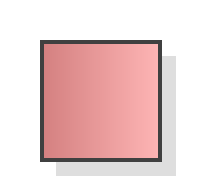
\includegraphics[width=2cm]{imageModelElementTeleportSource.png}
\vspace{-22pt}
\end{wrapfigure}

Siehe auch Abschnitt \textbf{Teleport-Transporte} im Lehrbuch.

Teleport-Transporte ermöglichen es, einen Kunden ohne Zeitverzug
von einem Teleport-Transport Startpunkt zu einem 
Teleport-Transport Zielpunkt (siehe Seite \pageref{ref:ModelElementTeleportDestination}) 
zu bewegen. Im Gegensatz zu normalen Transporten geht es hierbei nicht darum,
einen tatsächlichen Transport eines Kunden (der eine gewisse Zeit dauern und
Ressourcen benötigen kann) zu modellieren, sondern darum dass Modell übersichtlich
zu halten. Betritt ein Kunde einen Teleport-Transport Startpunkt, so wird er
augenblicklich zu dem dort angegeben Teleport-Transport Zielpunkt befördert.
Start- und Zielpunkt können sich an verschiedenen Stellen im Modell befinden;
im Gegensatz zu einem Transport über eine Kante wird keine Verbindunglinie
zwischen Start und Ziel eingezeichnet.

\subsection*{Einstellungen}

Der Name des Teleport-Transport Startpunktes besitzt keine weitere Bedeutung
für die Simulation. Allerdings muss der Name eines
Teleport-Transport Zielpunkt (siehe Seite \pageref{ref:ModelElementTeleportDestination}) 
Elements angegeben werden, zu dem die eintreffenden Kunden befördert werden sollen.


\section{Teleport-Transport Zielpunkt}
\label{ref:ModelElementTeleportDestination}

\begin{wrapfigure}{l}{2.5cm}
\vspace{-22pt}
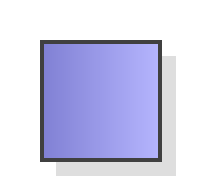
\includegraphics[width=2cm]{imageModelElementTeleportDestination.png}
\vspace{-22pt}
\end{wrapfigure}

Siehe auch Abschnitt \textbf{Teleport-Transporte} im Lehrbuch.

Teleport-Transporte ermöglichen es, einen Kunden ohne Zeitverzug
von einem Teleport-Transport Startpunkt (siehe Seite \pageref{ref:ModelElementTeleportSource}) 
zu einem Teleport-Transport Zielpunkt zu bewegen. Im Gegensatz zu normalen
Transporten geht es hierbei nicht darum, einen tatsächlichen Transport eines Kunden
(der eine gewisse Zeit dauern und Ressourcen benötigen kann) zu modellieren,
sondern darum dass Modell übersichtlich zu halten. Betritt ein Kunde einen
Teleport-Transport Startpunkt, so wird er augenblicklich zu dem dort angegeben
Teleport-Transport Zielpunkt befördert.
Start- und Zielpunkt können sich an verschiedenen Stellen im Modell befinden;
im Gegensatz zu einem Transport über eine Kante wird keine Verbindunglinie
zwischen Start und Ziel eingezeichnet.

\subsection*{Einstellungen}

Die Teleport-Transport Ziele werden über ihren Namen bei dem Transport der Kunden von
einem Teleport-Transport Startpunkt aus identifiziert.


\section{Transporter Wegpunkt}
\label{ref:ModelElementWayPoint}

\begin{wrapfigure}{l}{2.5cm}
\vspace{-22pt}

\includegraphics[width=2cm]{imageModelElementWayPoint.png}
\vspace{-22pt}
\end{wrapfigure}

Siehe auch Abschnitt \textbf{Transporte mit Transportern} im Lehrbuch.

Wegpunkte werden von Transportern während der Animation auf dem Weg von einer Ausgangs-
zu einer Zielstation angesteuert. Für die Simulation selbst besitzen sie keine Bedeutung.

\subsection*{Einstellungen}

Für jeden Wegpunkt kann eingestellt werden, bei dem Weg von welcher Ausgangs- zu welcher
Zielstation dieser angesteuert werden soll.

\textbf{Hinweis:}~\\
Das manuelle Erstellen von Wegstrecken direkt über die Einstellmöglichkeiten der
Wegpunkte ist sehr aufwendig. Um diesen Prozess zu vereinfachen, steht der
Wegstrecken-Editor , der über das Kontextmenü
eines Wegpunktes aufgerufen werden kann, zur Verfügung.


\section{Transportstart}
\label{ref:ModelElementTransportSource}

\begin{wrapfigure}{l}{2.5cm}
\vspace{-22pt}
\includegraphics[width=2cm]{imageModelElementTransportSource.png}
\vspace{-22pt}
\end{wrapfigure}

Siehe auch Abschnitt \textbf{Direkte Transporte} im Lehrbuch.

Ein Transportstartelement ermöglicht den Transport eines Kunden zu einem beliebigen
Transportziel-Element (siehe Seite \pageref{ref:ModelElementTransportDestination}) . Wie viel
Zeit der Transport beansprucht und zu welchem Zielelement der Kunde transportiert
wird, kann dabei in dem Transportstartelement eingestellt werden.
Für den Transport eines Kunden von einem Transportstart- zu einem Transportzielelement
muss keine Verbindungskante zwischen den Elementen bestehen.

\subsection*{Einstellungen}

Der Name des Transportstartelements besitzt keine weitere Bedeutung.

Auf der Dialogseite \textbf{Transportzeiten} kann festgelegt werden, wie lange der Transport
eines Kunden von diesem Transportstartelement zu dem jeweiligen Ziel dauern soll. Die Transportzeit
kann dabei als Verteilung oder als Ausdruck angegeben werden. Des Weiteren kann eingestellt
werden, ob die Transportzeit als Wartezeit, Transferzeit (Standard) oder Bedienzeit
erfasst werden soll.

Auf der Dialogseite \textbf{Transportziele} können ein oder mehrere
mögliche Ziel für den Transport des Kunden angegeben werden. Für die Ziele können dabei
Bedingungen oder Kundentypen angegeben werden. Alternativ kann eingestellt werden, dass
das anzusteuernde Ziel aus dem Fertigungsplan des Kunden oder aus einer Texteigenschaft
des Kunden entnommen werden soll.

Auf der Dialogseite \textbf{Benötigte Ressource} kann angegeben werden, ob
für den Transport eines Kunden eine Ressource benötigt. Neben dem Typ der
Ressource kann angegeben werden, wie viele Bediener der Ressource für den
Transport eines Kunden benötigt werden und ob die Ressource sofort nach dem
Eintreffen an der Zielstation freigegeben werden soll oder ggf. erst nach
einer bestimmten Verzögerungszeit (z.B. um die Rückfahrt der Ressource
zur Ausgangsstation zu modellieren).

Auf der Dialogseite \textbf{Bereich verlassen} kann optional eine
Bereich-betreten-Station angegeben werden. Beim Start des Transports
wird dann der angegebene Bereich verlassen.


\section{Transportziel}
\label{ref:ModelElementTransportDestination}

\begin{wrapfigure}{l}{2.5cm}
\vspace{-22pt}
\includegraphics[width=2cm]{imageModelElementTransportDestination.png}
\vspace{-22pt}
\end{wrapfigure}

Siehe auch Abschnitt \textbf{Direkte Transporte} im Lehrbuch.

Die Transportzielelemente können als Zielstationen für den Transport von Kunden von
Transportstart-Elementen (siehe Seite \pageref{ref:ModelElementTransportSource}) verwendet werden.
Für den Transport eines Kunden von einem Transportstart- zu einem Transportzielelement
muss keine Verbindungskante zwischen den Elementen bestehen.

\subsection*{Einstellungen}

Die Transportzielelemente werden über ihren Namen bei dem Routing der Kunden von
einem Transportstartelement identifiziert.


\section{Verzweigen und Teleportieren}
\label{ref:ModelElementDecideAndTeleport}

\begin{wrapfigure}{l}{2.5cm}
\vspace{-22pt}
\includegraphics[width=2cm]{imageModelElementDecideAndTeleport.png}
\vspace{-22pt}
\end{wrapfigure}

Teleport-Transporte ermöglichen es, einen Kunden ohne Zeitverzug
von einem Teleport-Transport Startpunkt zu einem 
Teleport-Transport Zielpunkt (siehe Seite \pageref{ref:ModelElementTeleportDestination}) 
zu bewegen. Im Gegensatz zu normalen Transporten geht es hierbei nicht darum,
einen tatsächlichen Transport eines Kunden (der eine gewisse Zeit dauern und
Ressourcen benötigen kann) zu modellieren, sondern darum dass Modell übersichtlich
zu halten. Betritt ein Kunde einen Teleport-Transport Startpunkt, so wird er
augenblicklich zu dem dort angegeben Teleport-Transport Zielpunkt befördert.
Start- und Zielpunkt können sich an verschiedenen Stellen im Modell befinden;
im Gegensatz zu einem Transport über eine Kante wird keine Verbindunglinie
zwischen Start und Ziel eingezeichnet.

Eine Verzweigen und Teleportieren Station kombiniert die Funktionalität
einer Verzweigen (siehe Seite \pageref{ref:ModelElementDecide}) -Station mit einer
Teleport-Transport Startpunkt (siehe Seite \pageref{ref:ModelElementTeleportSource}) -Station:
Zunächst wird das Kundenobjekt gemäß bestimmter Regeln in eine vorgegebene
Richtung geleitet. Dann wird es per Teleporttransport ohne Verbindungskante
zu diesem Ziel transportiert.

Die Verzweigung kann dabei nach folgenden Kriterien erfolgen:

\begin{itemize}
  \item 
    \textbf{Zufällig:}
    Pro Ausgangsrichtung wird eine Rate angegeben, die die Wahrscheinlichkeit für diesen Weg bestimmt.

  \item 
    \textbf{Bedingung:}
    Für alle Ausgangsrichtungen (außer für die letzte Richtung) wird eine Bedingung definiert. Trifft ein
    Kunde ein, so werden von oben nach unten diese Bedingungen geprüft. Der Kunde wird in die Richtung,
    bei der zum ersten Mal die Bedingung erfüllt war, weitergeleitet. Trifft keine der Bedingungen zu,
    so wird der Kunde in die letzte Richtung (für die keine Bedingung angegeben ist) weitergeleitet.    

  \item 
    \textbf{Kundentyp:}
    Für alle Ausgangsrichtungen (außer für die letzte Richtung) wird ein Kundentyp festgelegt. Ist ein
    eintreffender Kunde von einem dieser Typen, so wird er in die entsprechende Richtung weitergeleitet.
    Stimmt der Typ des eingetroffenen Kunden mit keinem der angegebenen Kundentypen überein,
    so wird der Kunde in die letzte Richtung (für die kein Kundentyp angegeben ist) weitergeleitet.

  \item 
    \textbf{Reihenfolge:}
    Es wird jeweils der Reihe nach einer der Kunden an einen der Ausgänge geleitet. Nachdem ein Kunde
    an den als letztes angebundenen Ausgang geleitet wurde, wird der nächste Kunde wieder an den
    ersten Ausgang geleitet. 

  \item 
    \textbf{Kürzeste Warteschlange an der nächsten Station:}
    Leitet den Kunden über den Pfad weiter, bei dem an der direkten Folgestation
    die Warteschlangenlänge minimal ist.

  \item 
    \textbf{Kürzeste Warteschlange an der nächsten Bedienstation:}
    Leitet den Kunden über den Pfad weiter, bei dem an der nächsten
    darin auftretenden Bedienstation die Warteschlangenlänge minimal ist.
    Andere Stationen, die zwischen dem Verzweigen-Element und der
    Bedienstation liegen, werden bei der Bestimmung der Warteschlangenlänge
    nicht berücksichtigt.

  \item 
    \textbf{Geringste Anzahl an Kunden an der nächsten Station:}
    Leitet den Kunden über den Pfad weiter, bei dem sich an der direkten Folgestation
    die geringste Anzahl an Kunden befinden.

  \item 
    \textbf{Geringste Anzahl an Kunden an der nächsten Bedienstation:}
    Leitet den Kunden über den Pfad weiter, bei dem sich an der nächsten
    darin auftretenden Bedienstation die geringste Anzahl an Kunden befinden.
    Andere Stationen, die zwischen dem Verzweigen-Element und der
    Bedienstation liegen, werden bei der Bestimmung der Anzahl an Kunden
    nicht berücksichtigt.

  \item 
    \textbf{Texteigenschaft:}
    Für alle Ausgangsrichtungen (außer für die letzte Richtung) wird ein Wert festgelegt.
    Wenn die Texteigenschaft des jeweiligen Kunden den jeweiligen Wert aufweist,
    so wird er in die entsprechende Richtung weitergeleitet.
    Stimmt der Wert mit keinem der angegebenen Wert überein,
    so wird der Kunde in die letzte Richtung (für die kein Wert angegeben ist) weitergeleitet.

\end{itemize}

\subsection*{Einstellungen}

\subsubsection*{Modus ,,Zufall''}

Die Weiterleitungswahrscheinlichkeiten in die verschiedenen möglichen Ausgangsrichtungen müssen nicht in
Form von Wahrscheinlichkeiten, die sich in ihrer Summe zu 1 aufaddieren müssen, angegeben werden, sondern
es genügt, Raten anzugeben. Diese Raten werden vom Programm automatisch zu Wahrscheinlichkeiten normiert.
Es gelten lediglich folgende Voraussetzungen: Die Raten dürfen nicht negativ sein und mindestens eine der
angegebenen Raten muss echt größer als 0 sein.

\subsubsection*{Modus ,,Bedingung''}

Pro vorhandener Verzweigung muss eine Bedingung angegeben werden, unter der die Kunden in diese Richtung
geleitet werden. Die Bedingungen müssen sich nicht gegenseitig ausschließen und werden von oben nach unten
abgearbeitet. Für die letzte Verzweigungsmöglichkeit kann keine Bedingung angegeben werden. Diese Verzweigung
wird in der Simulation immer dann gewählt, wenn keine der vorherigen Bedingungen zutreffend war.

\subsubsection*{Modus ,,Kundentyp''}

Pro vorhandener Verzweigung muss ein Kundentyp angegeben werden, dessen Kunden in diese Richtung
geleitet werden. Für die letzte Verzweigungsmöglichkeit kann kein Kundentyp angegeben werden. Diese Verzweigung
wird in der Simulation immer dann gewählt, wenn keine der vorherigen Bedingungen zutreffend war.

\subsubsection*{Modus ,,Texteigenschaft''}

Es muss ein Schlüssel, dessen Werte bei den Kunden betrachtet werden sollen, angegeben werden.
Außerdem muss pro vorhandener Verzweigung ein Wert angegeben werden. Kunden bei denen der Schlüssel
den angegebenen Wert besitzt, werden in diese Richtung geleitet. Für die letzte Verzweigungsmöglichkeit
kann kein Wert angegeben werden. Diese Verzweigung wird in der Simulation immer dann gewählt,
wenn keine der vorherigen Bedingungen zutreffend war.





\chapter{Daten Ein-/Ausgabe}

\section{Aufzeichnung}
\label{ref:ModelElementRecord}

\begin{wrapfigure}{l}{2.5cm}
\vspace{-22pt}
\includegraphics[width=2cm]{imageModelElementRecord.png}
\vspace{-22pt}
\end{wrapfigure}

Siehe auch Abschnitt \textbf{Datenaufzeichnung-Stationen} im Lehrbuch.

Durchläuft ein Kunde dieses Element, so werden die Werte von ein oder zwei frei definierbaren Ausdrücken
in der Statistik erfasst. Wird ein Ausdruck verwendet, so stehen die Werte später als Verlaufsdiagramm
zur Verfügung. Bei zwei Werten wird ein X-Y-Punktediagramm gebildet.

\subsection*{Einschränkungen}

Im Gegensatz zu der Aufzeichnung von Werten über ein Ausgabe-Element (siehe Seite \pageref{ref:ModelElementOutput}) 
direkt in eine Datei werden die Daten hier im Arbeitsspeicher gehalten, um im Anschluss an die Simulation
direkt in der Statistikansicht zur Verfügung zu stehen. Daher ist die Anzahl an Datenpunkten, die erfasst
werden auf 2 Millionen beschränkt. Beim Speichern der Statistikdaten als xml-Datei und bei der Anzeige eines
Verlaufsdiagramms werden diese maximal 2 Millionen Datenpunkte berücksichtigt. In X-Y-Punktediagrammen und
in Tabellen werden jedoch nur maximal 2$^{17}$ Datenpunkte ausgegeben.

\subsection*{Einstellungen}

Die Daten werden in der Statistik unter dem Namen des Datenaufzeichnung-Elements erfasst. Mindestens
ein Ausdruck, dessen Werte erfasst werden sollen, muss angegeben werden. Der zweite Ausdruck ist
optional.


\section{Ausgabe}
\label{ref:ModelElementOutput}

\begin{wrapfigure}{l}{2.5cm}
\vspace{-22pt}
\includegraphics[width=2cm]{imageModelElementOutput.png}
\vspace{-22pt}
\end{wrapfigure}

Siehe auch Abschnitt \textbf{Speichern von Werten während der Simulation} im Lehrbuch.

Durchläuft ein Kunde dieses Element, so wird eine Ausgabe von definierbaren Statusinformationen in eine
Datei angestoßen.

\subsection*{Einstellungen}

Der Name des Ausgabe-Elements hat keine weitere Bedeutung. Über das Dateinamefeld kann der Name der Datei,
in die die Daten geschrieben werden sollen, angegeben werden. Pro Kundenereignis können mehrere Daten
geschrieben werden, deren Reihenfolge und Werte über die Tabellenzeilen in dem Einstellungendialog zu
dem Ausgabe-Element definiert werden können.

\subsection*{Alternative}

Mit dem Ausgabe (JS)-Element (siehe Seite \pageref{ref:ModelElementOutputJS}) besteht die Möglichkeit, weit komplexere
Ausgabeformate für die Simulationsdaten zu definieren. Allerdings benötigt der Simulator für die Ausführung
des Ausgabe (JS)-Elements deutlich mehr Rechenzeit.


\section{Ausgabe (DB)}
\label{ref:ModelElementOutputDB}

\begin{wrapfigure}{l}{2.5cm}
\vspace{-22pt}
\includegraphics[width=2cm]{imageModelElementOutputDB.png}
\vspace{-22pt}
\end{wrapfigure}

Siehe auch Abschnitt \textbf{Speichern von Werten während der Simulation} im Lehrbuch.

Durchläuft ein Kunde dieses Element, so wird eine Ausgabe von definierbaren Statusinformationen in eine
Datenbanktabelle angestoßen.

\subsection*{Einstellungen}

Der Name des Ausgabe (DB) Elements hat keine weitere Bedeutung. Es müssen Verbindungsdaten zu einer
Datenbank sowie der Name der Tabelle in der Datenbank, in der die Daten gespeichert werden, angegeben werden.
Pro Kundenereignis können mehrere Daten in verschiedene Spalten geschrieben werden. Pro Kundenankunft
wird dabei eine neue Zeile in der Tabelle angelegt.


\section{Ausgabe (DDE)}
\label{ref:ModelElementOutputDDE}

\begin{wrapfigure}{l}{2.5cm}
\vspace{-22pt}
\includegraphics[width=2cm]{imageModelElementOutputDDE.png}
\vspace{-22pt}
\end{wrapfigure}

Siehe auch Abschnitt \textbf{Speichern von Werten während der Simulation} im Lehrbuch.

Durchläuft ein Kunde dieses Element, so wird eine Ausgabe von definierbaren Statusinformationen per
DDE in eine Excel-Tabelle geschrieben.

\subsection*{Einstellungen}

Der Name des Ausgabe (DDE) Elements hat keine weitere Bedeutung. Es müssen DDE-Verbindungseinstellungen
angegeben werden.
Pro Kundenereignis können mehrere Daten in verschiedene Spalten geschrieben werden. Pro Kundenankunft
wird dabei eine neue Zeile in der Tabelle angelegt.


\section{Ausgabe (Log)}
\label{ref:ModelElementOutputLog}

\begin{wrapfigure}{l}{2.5cm}
\vspace{-22pt}
\includegraphics[width=2cm]{imageModelElementOutputLog.png}
\vspace{-22pt}
\end{wrapfigure}

Siehe auch Abschnitt \textbf{Speichern von Werten während der Simulation} im Lehrbuch.

Durchläuft ein Kunde dieses Element, so wird eine Ausgabe von definierbaren Statusinformationen in
die Logging-Ausgabe angestoßen. Ist das Logging nicht aktiviert, so erfolgt keine Ausgabe.

\subsection*{Einstellungen}

Der Name des Ausgabe-Elements hat keine weitere Bedeutung. Pro Kundenereignis können mehrere Daten
geschrieben werden, deren Reihenfolge und Werte über die Tabellenzeilen in dem Einstellungendialog zu
dem Ausgabe-Element definiert werden können.


\section{Ausgabe (Skript)}
\label{ref:ModelElementOutputJS}

\begin{wrapfigure}{l}{2.5cm}
\vspace{-22pt}
\includegraphics[width=2cm]{imageModelElementOutputJS.png}
\vspace{-22pt}
\end{wrapfigure}

Siehe auch Abschnitt \textbf{Speichern von Werten während der Simulation} im Lehrbuch.

Durchläuft ein Kunde dieses Element, so wird eine Ausgabe von über ein Javascript-
oder ein Java-Programm definierbaren Statusinformationen in eine Datei angestoßen.

\subsection*{Einstellungen}

Der Name des Ausgabe-Elements hat keine weitere Bedeutung. Über das Dateinamefeld kann der Name der Datei,
in die die Daten geschrieben werden sollen, angegeben werden. Die auszuführenden Skriptbefehle werden in
\textbf{Javascript} oder in \textbf{Java} angegeben. Zusätzlich stehen einige
besondere Javascript-Befehle bzw. besondere Java-Befehle 
zum Zugriff auf die Simulationsdaten zur Verfügung.

\subsection*{Alternative}

Die Definition der Ausgaben in Form eines Javascript- oder eines Java-Programms erlaubt eine größtmögliche Flexibilität,
benötigt jedoch verhältnismäßig viel Zeit. Eine schnellere Möglichkeit zur Ausgabe von Simulationsdaten
bietet das Ausgabe-Element (siehe Seite \pageref{ref:ModelElementOutput}) .


\section{Eingabe}
\label{ref:ModelElementInput}

\begin{wrapfigure}{l}{2.5cm}
\vspace{-22pt}
\includegraphics[width=2cm]{imageModelElementInput.png}
\vspace{-22pt}
\end{wrapfigure}

Siehe auch Abschnitt \textbf{Laden von Werten während der Simulation} im Lehrbuch.

Durchläuft ein Kunde dieses Element, so wird eine Zahl aus einer Datei gelesen und einer
Variable zugewiesen. Die Leseposition in der Datei wird dabei um eine Zeile weiter bewegt.
Wird durch einen Kunden das Dateiende erreicht, so kann eingestellt werden, wie sich
das Element verhalten soll.

\subsection*{Einstellungen}

Der Name des Eingabe-Elements besitzt keine weitere Bedeutung. Es müssen der Name der zu lesenden
Datei, das gewünschte Verhalten am Dateiende sowie der Name der Variable, an die die Zuweisungen
erfolgen sollen, eingestellt werden.

Über die drei Pseudo-Variablennamen ,,w'', ,,t'' und ,,p'' kann lesend und schreibend auf die Wartezeit, die Transferzeit
und die Bedienzeit des aktuellen Kunden (jeweils auf Sekundenbasis) zugegriffen werden. Außerdem kann statt eines
Variablennamens ein Kundenobjekt-Datenfeld über ,,ClientData(index)'' beschrieben werden oder über ,,ClientData('Schlüssel')"
ein Textwert in einem kundenbasierenden Schlüssel hinterlegt werden.

\subsection*{Alternative}

Mit dem Eingabe (JS)-Element (siehe Seite \pageref{ref:ModelElementInputJS}) besteht die Möglichkeit, weit komplexere
Verarbeitungen auf Basis der Eingabewerte vorzunehmen. Allerdings benötigt der Simulator für die Ausführung
des dann zugehörigen Javascript-Elements deutlich mehr Rechenzeit.


\section{Eingabe (DB)}
\label{ref:ModelElementInputDB}

\begin{wrapfigure}{l}{2.5cm}
\vspace{-22pt}
\includegraphics[width=2cm]{imageModelElementInputDB.png}
\vspace{-22pt}
\end{wrapfigure}

Siehe auch Abschnitt \textbf{Laden von Werten während der Simulation} im Lehrbuch.

Durchläuft ein Kunde dieses Element, so wird eine Zahl aus einer Datenbanktabelle gelesen und einer
Variable zugewiesen. Die Leseposition in der Tabelle wird dabei um eine Zeile weiter bewegt.
Wird durch einen Kunden das Dateiende erreicht, so kann eingestellt werden, wie sich
das Element verhalten soll.

\subsection*{Einstellungen}

Der Name des Eingabe-Elements besitzt keine weitere Bedeutung. Neben den Verbindungseinstellungen
zur Datenbank und der Auswahl von Tabelle und Spalte müssen das gewünschte Verhalten am Tabellenende
sowie der Name der Variable, an die die Zuweisungen erfolgen sollen, eingestellt werden.

Über die drei Pseudo-Variablennamen ,,w'', ,,t'' und ,,p'' kann lesend und schreibend auf die Wartezeit, die Transferzeit
und die Bedienzeit des aktuellen Kunden (jeweils auf Sekundenbasis) zugegriffen werden. Außerdem kann statt eines
Variablennamens ein Kundenobjekt-Datenfeld über ,,ClientData(index)'' beschrieben werden oder über ,,ClientData('Schlüssel')"
ein Textwert in einem kundenbasierenden Schlüssel hinterlegt werden.


\section{Eingabe (DDE)}
\label{ref:ModelElementInputDDE}

\begin{wrapfigure}{l}{2.5cm}
\vspace{-22pt}
\includegraphics[width=2cm]{imageModelElementInputDDE.png}
\vspace{-22pt}
\end{wrapfigure}

Siehe auch Abschnitt \textbf{Laden von Werten während der Simulation} im Lehrbuch.

Durchläuft ein Kunde dieses Element, so wird eine Zahl per DDE aus einer Excel-Tabelle gelesen und einer
Variable zugewiesen. Die Leseposition in der Tabelle wird dabei um eine Zeile weiter bewegt.
Wird durch einen Kunden das Dateiende erreicht, so kann eingestellt werden, wie sich
das Element verhalten soll.

\subsection*{Einstellungen}

Der Name des Eingabe-Elements besitzt keine weitere Bedeutung. Neben den DDE-Verbindungseinstellungen
müssen das gewünschte Verhalten am Tabellenende
sowie der Name der Variable, an die die Zuweisungen erfolgen sollen, eingestellt werden.

Über die drei Pseudo-Variablennamen ,,w'', ,,t'' und ,,p'' kann lesend und schreibend auf die Wartezeit, die Transferzeit
und die Bedienzeit des aktuellen Kunden (jeweils auf Sekundenbasis) zugegriffen werden. Außerdem kann statt eines
Variablennamens ein Kundenobjekt-Datenfeld über ,,ClientData(index)'' beschrieben werden oder über ,,ClientData('Schlüssel')"
ein Textwert in einem kundenbasierenden Schlüssel hinterlegt werden.


\section{Eingabe (Skript)}
\label{ref:ModelElementInputJS}

\begin{wrapfigure}{l}{2.5cm}
\vspace{-22pt}
\includegraphics[width=2cm]{imageModelElementInputJS.png}
\vspace{-22pt}
\end{wrapfigure}

Siehe auch Abschnitt \textbf{Laden von Werten während der Simulation} im Lehrbuch.

Durchläuft ein Kunde dieses Element, so wird eine Zahl aus einer Datei gelesen und in
einem nutzerdefinierten Javascript- oder Java-Programm zur Verfügung gestellt. 

\subsection*{Einstellungen}

Der Name des Eingabe-Elements besitzt keine weitere Bedeutung. Es müssen der Name der zu lesenden
Datei, das gewünschte Verhalten am Dateiende sowie das auszuführende Skript angegeben werden.
Die auszuführenden Skriptbefehle werden in \textbf{Javascript} oder in \textbf{Java} angegeben.
Zusätzlich stehen einige besondere Javascript-Befehle bzw.
die besondere Java-Befehle 
zum Zugriff auf die Simulationsdaten zur Verfügung.

\subsection*{Alternative}

Die Definition von Zuweisungen in Form eines Javascript- oder eines Java-Programms erlaubt eine größtmögliche Flexibilität,
benötigt jedoch verhältnismäßig viel Zeit. Eine schnellere Möglichkeit zur Zuweisung von Variablen
bietet das Eingabe-Element (siehe Seite \pageref{ref:ModelElementInput}) .





\chapter{Flusssteuerungslogik}

\section{Do}
\label{ref:ModelElementLogicDo}

\begin{wrapfigure}{l}{2.5cm}
\vspace{-22pt}
\includegraphics[width=2cm]{imageModelElementLogicDo.png}
\vspace{-22pt}
\end{wrapfigure}

Siehe auch Abschnitt \textbf{Flusssteuerung} im Lehrbuch.

Das Do-Element leitet den Kunden immer zum direkt folgenden Element weiter.
Es dient als Schleifenanfang bzw. als Sprungziel für
Until (siehe Seite \pageref{ref:ModelElementLogicUntil}) -Stationen.

\subsection*{Einstellungen}

Der Name der Station besitzt keine Bedeutung für die Simulation.


\section{Else}
\label{ref:ModelElementLogicElse}

\begin{wrapfigure}{l}{2.5cm}
\vspace{-22pt}
\includegraphics[width=2cm]{imageModelElementLogicElse.png}
\vspace{-22pt}
\end{wrapfigure}

Siehe auch Abschnitt \textbf{Flusssteuerung} im Lehrbuch.

Das Else-Element leitet den Kunden in Abhängigkeit davon, ob die Bedingung an einem
vorhergehenden If (siehe Seite \pageref{ref:ModelElementLogicIf}) - oder
ElseIf-Element (siehe Seite \pageref{ref:ModelElementLogicElseIf}) erfüllt ist, entweder
zur unmittelbar nächsten Station weiter (wenn die Bedingung nicht erfüllt ist) oder
zur folgenden EndIf (siehe Seite \pageref{ref:ModelElementLogicEndIf}) -Station.
Dies ermöglicht eine grafische Variante einer Flusssteuerung wie sie bei
klassischen Programmiersprachen vorhanden ist.

\subsection*{Einstellungen}

Der Name der Station besitzt keine Bedeutung für die Simulation.


\section{ElseIf}
\label{ref:ModelElementLogicElseIf}

\begin{wrapfigure}{l}{2.5cm}
\vspace{-22pt}
\includegraphics[width=2cm]{imageModelElementLogicElseIf.png}
\vspace{-22pt}
\end{wrapfigure}

Siehe auch Abschnitt \textbf{Flusssteuerung} im Lehrbuch.

Das ElseIf-Element leitet den Kunden in Abhängigkeit davon, ob die Bedingung
an einem vorhergehenden If (siehe Seite \pageref{ref:ModelElementLogicIf}) - oder
ElseIf-Element (siehe Seite \pageref{ref:ModelElementLogicElseIf}) erfüllt ist
sowie in Abhängigkeit von einer Bedienung (wenn die Bedingung an den vorherigen
Elementen nicht erfüllt war) entweder zur unmittelbar nächsten Station weiter
(wenn die Bedingung erfüllt ist) oder zu einer folgenden
ElseIf (siehe Seite \pageref{ref:ModelElementLogicElseIf}) -,
Else (siehe Seite \pageref{ref:ModelElementLogicElse}) - oder
EndIf (siehe Seite \pageref{ref:ModelElementLogicEndIf}) -Station.
Dies ermöglicht eine grafische Variante einer Flusssteuerung wie sie bei
klassischen Programmiersprachen vorhanden ist.

\subsection*{Einstellungen}

Der Name der Station besitzt keine Bedeutung für die Simulation. Über die Bedingung
wird gesteuert, zu welcher Station die jeweiligen Kunden weitergeleitet werden.


\section{EndIf}
\label{ref:ModelElementLogicEndIf}

\begin{wrapfigure}{l}{2.5cm}
\vspace{-22pt}
\includegraphics[width=2cm]{imageModelElementLogicEndIf.png}
\vspace{-22pt}
\end{wrapfigure}

Siehe auch Abschnitt \textbf{Flusssteuerung} im Lehrbuch.

Das EndIf-Element beendet eine durch ein
If-Element (siehe Seite \pageref{ref:ModelElementLogicEndIf}) eingeleitete
Flusssteuerungskette.

\subsection*{Einstellungen}

Der Name der Station besitzt keine Bedeutung für die Simulation.


\section{EndWhile}
\label{ref:ModelElementLogicEndWhile}

\begin{wrapfigure}{l}{2.5cm}
\vspace{-22pt}
\includegraphics[width=2cm]{imageModelElementLogicEndWhile.png}
\vspace{-22pt}
\end{wrapfigure}

Siehe auch Abschnitt \textbf{Flusssteuerung} im Lehrbuch.

Das EndWhile-Element beendet eine mit einem
While-Element (siehe Seite \pageref{ref:ModelElementLogicWhile}) begonnene
Schleife. Der Kunde wird an das While-Element zurück verwiesen.
Dieses prüft, ob die Bedingung nach wie vor erfüllt ist.
Wenn nein, wird der Kunde an das auf dieses EndWhile-Element
folgende Element geleitet. Ansonsten wird die Schleife ein
weiteres Mal durchlaufen.

\subsection*{Einstellungen}

Der Name der Station besitzt keine Bedeutung für die Simulation.


\section{If}
\label{ref:ModelElementLogicIf}

\begin{wrapfigure}{l}{2.5cm}
\vspace{-22pt}
\includegraphics[width=2cm]{imageModelElementLogicIf.png}
\vspace{-22pt}
\end{wrapfigure}

Siehe auch Abschnitt \textbf{Flusssteuerung} im Lehrbuch.

Das If-Element leitet den Kunden in Abhängigkeit von einer Bedingung entweder
zur unmittelbar nächsten Station weiter (wenn die Bedingung erfüllt ist) oder
zu einer folgenden ElseIf (siehe Seite \pageref{ref:ModelElementLogicElseIf}) -,
Else (siehe Seite \pageref{ref:ModelElementLogicElse}) - oder
EndIf (siehe Seite \pageref{ref:ModelElementLogicEndIf}) -Station.
Dies ermöglicht eine grafische Variante einer Flusssteuerung wie sie bei
klassischen Programmiersprachen vorhanden ist.

\subsection*{Einstellungen}

Der Name der Station besitzt keine Bedeutung für die Simulation. Über die Bedingung
wird gesteuert, zu welcher Station die jeweiligen Kunden weitergeleitet werden.


\section{Until}
\label{ref:ModelElementLogicUntil}

\begin{wrapfigure}{l}{2.5cm}
\vspace{-22pt}
\includegraphics[width=2cm]{imageModelElementLogicUntil.png}
\vspace{-22pt}
\end{wrapfigure}

Siehe auch Abschnitt \textbf{Flusssteuerung} im Lehrbuch.

Das Until-Element beendet eine mit einem
Do-Element (siehe Seite \pageref{ref:ModelElementLogicDo}) begonnene
Schleife. Der Kunde wird an das Do-Element zurück verwiesen,
sofern die Bedingung noch nicht erfüllt ist.

\subsection*{Einstellungen}

Der Name der Station besitzt keine Bedeutung für die Simulation.
Über die Bedingung wird gesteuert, zu welcher Station die jeweiligen Kunden weitergeleitet werden.


\section{While}
\label{ref:ModelElementLogicWhile}

\begin{wrapfigure}{l}{2.5cm}
\vspace{-22pt}
\includegraphics[width=2cm]{imageModelElementLogicWhile.png}
\vspace{-22pt}
\end{wrapfigure}

Siehe auch Abschnitt \textbf{Flusssteuerung} im Lehrbuch.

Das While-Element leitet den Kunden in Abhängigkeit von einer Bedingung entweder
zur unmittelbar nächsten Station weiter (wenn die Bedingung erfüllt ist) oder
zur folgenden EndWhile (siehe Seite \pageref{ref:ModelElementLogicEndWhile}) -Station.
Dies ermöglicht eine grafische Variante einer Flusssteuerung wie sie bei
klassischen Programmiersprachen vorhanden ist.

\subsection*{Einstellungen}

Der Name der Station besitzt keine Bedeutung für die Simulation. Über die Bedingung
wird gesteuert, zu welcher Station die jeweiligen Kunden weitergeleitet werden.





\chapter{Analoge Werte}

\section{Analogen W. ändern}
\label{ref:ModelElementAnalogAssign}

\begin{wrapfigure}{l}{2.5cm}
\vspace{-22pt}
\includegraphics[width=2cm]{imageModelElementAnalogAssign.png}
\vspace{-22pt}
\end{wrapfigure}

Siehe auch Abschnitt \textbf{Analoger-Wert-Stationen} im Lehrbuch.

Passiert ein Kunde dieses Element, so werden in einem oder mehreren
Analoger Wert (siehe Seite \pageref{ref:ModelElementAnalogValue}) - und
Tank-Elementen (siehe Seite \pageref{ref:ModelElementTank}) 
neue Werte und Änderungsraten eingetragen.

\subsection*{Einstellungen}

Der Name des ,,Analogen Wert ändern''-Elements besitzt keine weitere Bedeutung für die Simulation.
Es kann eingestellt werden, in welchen Elementen welche Werte oder Raten verändert werden sollen.


\section{Analoger Wert}
\label{ref:ModelElementAnalogValue}

\begin{wrapfigure}{l}{2.5cm}
\vspace{-22pt}
\includegraphics[width=2cm]{imageModelElementAnalogValue.png}
\vspace{-22pt}
\end{wrapfigure}

Siehe auch Abschnitt \textbf{Analoger-Wert-Stationen} im Lehrbuch.

Dieses Element hält einen Wert, der sich gemäß einer bestimmten Rate über die Zeit ändert, vor.
Der Wert und die Rate können zur Laufzeit über ein
Analogen Wert ändern-Element (siehe Seite \pageref{ref:ModelElementAnalogAssign}) verändert werden.

Wenn ein Minimal- und ein Maximalwert für den Wert eingestellt sind, wird in das Element
selbst der \textbf{Füllstand} eingezeichnet.

\subsection*{Einstellungen}

Der Name des ,,Analoger Wert''-Elements besitzt keine weitere Bedeutung für die Simulation.
Neben dem initialen Wert, der initialen Änderungsrate sowie optionalen Minimum- und Maximumwerten
kann eingestellt werden, wie häufig die diskret verlaufende Simulation über die kontinuierliche
erfolgende Veränderung des Wertes benachrichtigt werden soll.


\section{Fluss}
\label{ref:ModelElementTankFlowByClient}

\begin{wrapfigure}{l}{2.5cm}
\vspace{-22pt}
\includegraphics[width=2cm]{imageModelElementTankFlowByClient.png}
\vspace{-22pt}
\end{wrapfigure}

Siehe auch Abschnitt \textbf{Tank-Stationen} im Lehrbuch.

Ein Fluss stellt eine Verbindung zwischen zwei Tanks (siehe Seite \pageref{ref:ModelElementTank}) 
(genauer zwischen zwei Ventilen an verschiedenen Tanks) dar.
Oder zwischen einer Fluss-Quelle und einem Tank oder zwischen einem Tank und einer Fluss-Senke.

Ein Fluss definiert, wie viele Einheiten von der Quelle zum Ziel fließen sollen oder wie
lange der Fluss aktiv sein soll.

Aktiviert wird der Fluss durch einen durch einen Kunden, der das Element erreicht.

\subsection*{Einstellungen}

Der Name des ,,Fluss''-Elements besitzt keine weitere Bedeutung für die Simulation.
Bei jedem Fluss müssen eine Quelle und ein Ziel angegeben werden.
Außerdem muss definiert werden, wie lange der Fluss aktiv sein soll. Als Aktivitätsdauer
können eine Zeitspanne, eine Durchflussmenge oder ein Stopp-Signal definiert werden.


\section{Fluss (Signal)}
\label{ref:ModelElementTankFlowBySignal}

\begin{wrapfigure}{l}{2.5cm}
\vspace{-22pt}
\includegraphics[width=2cm]{imageModelElementTankFlowBySignal.png}
\vspace{-22pt}
\end{wrapfigure}

Siehe auch Abschnitt \textbf{Tank-Stationen} im Lehrbuch.

Ein Fluss stellt eine Verbindung zwischen zwei Tanks (siehe Seite \pageref{ref:ModelElementTank}) 
(genauer zwischen zwei Ventilen an verschiedenen Tanks) dar.
Oder zwischen einer Fluss-Quelle und einem Tank oder zwischen einem Tank und einer Fluss-Senke.

Ein Fluss definiert, wie viele Einheiten von der Quelle zum Ziel fließen sollen oder wie
lange der Fluss aktiv sein soll.

Aktiviert wird der Fluss durch ein Signal.

\subsection*{Einstellungen}

Der Name des ,,Fluss''-Elements besitzt keine weitere Bedeutung für die Simulation.
Es muss angegeben werden, durch welches Signal der Fluss ausgelöst werden soll.
Außerdem müssen jedem Fluss müssen eine Quelle und ein Ziel angegeben werden und es muss
definiert werden, wie lange der Fluss aktiv sein soll. Als Aktivitätsdauer
können eine Zeitspanne, eine Durchflussmenge oder ein Stopp-Signal definiert werden.


\section{Sensor}
\label{ref:ModelElementTankSensor}

\begin{wrapfigure}{l}{2.5cm}
\vspace{-22pt}
\includegraphics[width=2cm]{imageModelElementTankSensor.png}
\vspace{-22pt}
\end{wrapfigure}

Siehe auch Abschnitt \textbf{Tank-Stationen} im Lehrbuch.

Ein Sensor-Element löst, vergleichbar einem Signal-Element (siehe Seite \pageref{ref:ModelElementSignal}) ,
ein Signal aus. Allerdings wird das Signal nicht ausgelöst, wenn ein Kunde das Element
passiert, sondern wenn bei einem zugehörigen Tank-Element (siehe Seite \pageref{ref:ModelElementTank}) 
ein bestimmter Füllstand über- oder unterschritten wird. 

\subsection*{Einstellungen}

Der Name des Sensor-Elements ist gleichzeitig der Name des Signal, das ausgelöst wird, wenn die Bedingung erfüllt ist.
Als Bedingung kann entweder die Über- oder Unterschreitung eines bestimmten Füllstandes in einem
Tank verwendet werden.


\section{Tank}
\label{ref:ModelElementTank}

\begin{wrapfigure}{l}{2.5cm}
\vspace{-22pt}
\includegraphics[width=2cm]{imageModelElementTank.png}
\vspace{-22pt}
\end{wrapfigure}

Siehe auch Abschnitt \textbf{Tank-Stationen} im Lehrbuch.

Dieses Element hält einen Wert, der sich gemäß bestimmter Raten über die Zeit ändert, vor.
Jeder Tank verfügt über ein oder mehrere Ventile. An diese Ventile können Flüsse
(siehe Fluss (siehe Seite \pageref{ref:ModelElementTankFlowByClient}) - und
Fluss (Signal)-Elemente (siehe Seite \pageref{ref:ModelElementTankFlowBySignal}) ) angeschlossen werden.
Die Ventile geben vor, wie viel Einheiten des Tankinhalts pro Zeiteinheit durch diese
fließen können, die Flüsse geben vor, wie viel Einheiten transportiert werden sollen oder
wie lange der Fluss aktiv sein soll.

Im Gegensatz zu den Analoger Wert-Elementen (siehe Seite \pageref{ref:ModelElementAnalogValue}) 
kann der Wert nicht negativ sein und es ist immer eine obere Grenze (die Kapazität des Tanks)
anzugeben.

An ein Ventil muss nicht zu jedem Zeitpunkt ein Fluss angedockt werden.
Ist ein Fluss an ein Ventil angedockt, so wird dieser direkt bedient.
Sind mehrere Flüsse angedockt, so wird zu jeder Zeit immer nur ein Fluss bedient.
Erst wenn der zeitlich zu erst eingetroffene Fluss abgearbeitet wurde, wird der nächste
aktiviert. D.h. es ist nicht so, dass mehrere Flüsse sich die verfügbare Durchflussmenge
eines Ventils auf irgendeine Weise teilen.

\subsection*{Einstellungen}

Der Name des ,,Tank''-Elements besitzt keine weitere Bedeutung für die Simulation.
Neben der Kapazität, dem initialen Wert und den Ventile mit ihren maximalen Durchflüssen
pro Zeiteinheit kann eingestellt werden, wie häufig die diskret verlaufende Simulation über die kontinuierliche
erfolgende Veränderung des Wertes benachrichtigt werden soll.


\section{Ventil-Setup}
\label{ref:ModelElementTankValveSetup}

\begin{wrapfigure}{l}{2.5cm}
\vspace{-22pt}
\includegraphics[width=2cm]{imageModelElementTankValveSetup.png}
\vspace{-22pt}
\end{wrapfigure}

Siehe auch Abschnitt \textbf{Tank-Stationen} im Lehrbuch.

Passiert ein Kunde ein Ventil-Setup-Element, so werden die maximalen Durchflüsse an einem
oder mehreren Ventilen an Tank-Elementen (siehe Seite \pageref{ref:ModelElementTank}) geändert.

\subsection*{Einstellungen}

Der Name des ,,Ventil-Setup''-Elements besitzt keine weitere Bedeutung für die Simulation.
Es können beliebige viele Ventile angegeben werden, die auf einen neuen maximalen Durchfluss
eingestellt werden sollen.





\chapter{Animation}

\section{Alarm}
\label{ref:ModelElementAnimationAlarm}

\begin{wrapfigure}{l}{2.5cm}
\vspace{-22pt}
\includegraphics[width=2cm]{imageModelElementAnimationAlarm.png}
\vspace{-22pt}
\end{wrapfigure}

Passiert ein Kunde im Animations-Modus ein Alarm-Element, so wird ein nutzerdefinierter Sound abgespielt.
Im Simulations-Modus führt ein Alarm-Element keine Handlungen aus.

\subsection*{Einstellungen}

Der Name des ,,Alarm''-Elements besitzt keine weitere Bedeutung für die Simulation.
Es kann eingestellt werden, unter welchen Bedingungen die Sound-Ausgabe erfolgen soll
und welche Sound-Datei bzw. welcher System-Sound abgespielt werden soll,
wenn ein Kunde die Station im Animations-Modus erreicht.


\section{Analogskalaanzeige}
\label{ref:ModelElementAnimationPointerMeasuring}

\begin{wrapfigure}{l}{2.5cm}
\vspace{-22pt}
\includegraphics[width=2cm]{imageModelElementAnimationPointerMeasuring.png}
\vspace{-22pt}
\end{wrapfigure}

Siehe auch Abschnitt \textbf{Animation von Modellen} im Lehrbuch.

Ein Analogskalaanzeige-Element ermöglicht es, den aktuellen Wert eines Rechenausdrucks
durch die Zeigerstellung auf einer analogen Messskala darzustellen.

\subsection*{Einstellungen}

Der Name des Elements besitzt keine weitere Bedeutung.
Zusätzlich zu dem auszuwertenden Rechenausdruck muss
der Maximalwert der Skala angegeben werden. Außerdem können
optional ein gelber und ein roter Bereich (typischerweise
mit Werten dicht unter dem Maximum) angegeben werden. Die
entsprechenden Bereiche werden dann farbig markiert auf
der Skala angezeigt.


\section{Animationsbild}
\label{ref:ModelElementAnimationImage}

\begin{wrapfigure}{l}{2.5cm}
\vspace{-22pt}
\includegraphics[width=2cm]{imageModelElementAnimationImage.png}
\vspace{-22pt}
\end{wrapfigure}

Siehe auch Abschnitt \textbf{Animation von Modellen} im Lehrbuch.

In dem Animationsbildelement können mehrere Bilder hinterlegt werden, die während der
Animation des Modells in Abhängigkeit von besimmten per Ausdruck festlegbaren
Bedingungen angezeigt werden.

\subsection*{Einstellungen}

Der Name des Animationsbildelement-Elements besitzt keine weitere Bedeutung. 
Zu jedem Bild kann eine Bedigung festgelegt werden. Die Liste der Bilder und
Bedingungen wird während der Animation stets von oben nach unten abgearbeitet.
Das Bild, welches zu der ersten zutreffenden Bedingung gehört, wird angezeigt.
Trifft keine der angegebenen Bedingungen zu, so wird das letzte Bild in der
Liste (zu dem keine Bedingung angegeben werden kann) angezeigt.


\section{Datenaufzeichnung anzeigen}
\label{ref:ModelElementAnimationRecord}

\begin{wrapfigure}{l}{2.5cm}
\vspace{-22pt}
\includegraphics[width=2cm]{imageModelElementAnimationRecord.png}
\vspace{-22pt}
\end{wrapfigure}

Siehe auch Abschnitt \textbf{Animation von Modellen} im Lehrbuch.

Stationen vom Typ ,,Datenaufzeichnung anzeigen'' dienen dazu, Werte die an
Datenaufzeichnung (siehe Seite \pageref{ref:ModelElementRecord}) -Stationen erfasst
wurden, während der Animation anzuzeigen. Die Anzeigeform (Liniendiagramm oder
X-Y-Punktediagramm) wird dabei gemäß dem Typ der Datenaufzeichnung (ein oder zwei Werte)
automatisch gewählt.

\subsection*{Einstellungen}

Der Name des Datenaufzeichnung anzeigen Elements besitzt keine weitere Bedeutung.
Zur Anzeige von Daten muss ein Datenaufzeichnung-Elemente, von dem die Daten
übernommen werden sollen, angegeben werden und es muss eingestellt werden, wie
viele Datenpunkte jeweils berücksichtigt werden sollen. (Es werden stets die neusten
erfassten Daten angezeigt).


\section{Icon: Person - Blau}
\label{ref:ModelElementClientIcon}

\begin{wrapfigure}{l}{2.5cm}
\vspace{-22pt}
\includegraphics[width=2cm]{imageModelElementClientIcon.png}
\vspace{-22pt}
\end{wrapfigure}

Das Icon-Element weist den Kunden, die es passieren, ein neues Animationsicon zu.

\subsection*{Einstellungen}

Der Name des Icon-Elements hat keine weitere Bedeutung. Über das Icon-Auswahlfeld kann das Icon,
welches den Kunden beim Passieren dieses Elements zugewiesen werden soll, ausgewählt werden.

Die optionale Bedingung ermöglicht es, dass nur unter bestimmten Voraussetzungen eine Zuweisung erfolgt,
wenn ein Kunde die Station passiert.


\section{LCD-Anzeige}
\label{ref:ModelElementAnimationLCD}

\begin{wrapfigure}{l}{2.5cm}
\vspace{-22pt}
\includegraphics[width=2cm]{imageModelElementAnimationLCD.png}
\vspace{-22pt}
\end{wrapfigure}

Siehe auch Abschnitt \textbf{Animation von Modellen} im Lehrbuch.

Ein LCD-Anzeige-Element ermöglicht es, den aktuellen Wert eines Rechenausdrucks
in Form eine 7-Segmentanzeige mit einstellbarer Anzeige an Ziffern darzustellen.
Ausgegeben wird dabei jeweils nur der Ganzzahlanteil des Wertes.

\subsection*{Einstellungen}

Der Name des Elements besitzt keine weitere Bedeutung.
Zusätzlich zu dem auszuwertenden Rechenausdruck können
die Anzahl an anzuzeigenden 7-Segment-Ziffern und die
Farbe der aktiven Segment eingestellt werden.


\section{Simulationsdaten als Balken}
\label{ref:ModelElementAnimationBar}

\begin{wrapfigure}{l}{2.5cm}
\vspace{-22pt}
\includegraphics[width=2cm]{imageModelElementAnimationBar.png}
\vspace{-22pt}
\end{wrapfigure}

Siehe auch Abschnitt \textbf{Animation von Modellen} im Lehrbuch.

Das Simulationsdaten als Balken Element ermöglicht es, während der Animation eines Modells laufend den Wert
eines Ausdrucks in Form eines verschieden großen Balken anzuzeigen. Angezeigt werden kann dabei jeder berechenbare
Ausdruck (was die Funktionen zur Bestimmung der Warteschlangenlängen an einzelnen Stationen genauso mit einschließt
wie der Zugriff auf alle nutzerdefinierten Simulations-Variablen). Für die klassische Simulation sind die
Simulationsdaten-Elemente ohne weitere Bedeutung.

\subsection*{Einstellungen}

Der Name des Simulationsdaten-Elements besitzt keine weitere Bedeutung. Für den darzustellenden Ausdruck kann
ein Bereich eingestellt werden, den der Balken repräsentieren soll.


\section{Simulationsdaten als gestapelter Balken}
\label{ref:ModelElementAnimationBarStack}

\begin{wrapfigure}{l}{2.5cm}
\vspace{-22pt}
\includegraphics[width=2cm]{imageModelElementAnimationBarStack.png}
\vspace{-22pt}
\end{wrapfigure}

Siehe auch Abschnitt \textbf{Animation von Modellen} im Lehrbuch.

Das Simulationsdaten als gestapelter Balken Element ermöglicht es, während der Animation eines Modells laufend die Werte
mehrerer Ausdrücke in Form eines Balkens, der aus mehreren Segmenten besteht, anzuzeigen. Angezeigt werden können dabei
alle berechenbaren Ausdrücke (was die Funktionen zur Bestimmung der Warteschlangenlängen an einzelnen Stationen genauso
mit einschließt wie der Zugriff auf alle nutzerdefinierten Simulations-Variablen). Für die klassische Simulation sind die
Simulationsdaten-Elemente ohne weitere Bedeutung.

\subsection*{Einstellungen}

Der Name des Simulationsdaten-Elements besitzt keine weitere Bedeutung.
Für die Summe der darzustellenden Werte kann ein Maximalwert angegeben werden.
Wird kein Maximalwert vorgegeben, so werden die Teilbalken so skaliert,
dass Sie die Gesamtfläche stets ausfüllen.


\section{Simulationsdaten als Text}
\label{ref:ModelElementAnimationText}

\begin{wrapfigure}{l}{2.5cm}
\vspace{-22pt}
\includegraphics[width=2cm]{imageModelElementAnimationText.png}
\vspace{-22pt}
\end{wrapfigure}

Siehe auch Abschnitt \textbf{Animation von Modellen} im Lehrbuch.

Das Simulationsdaten als Text Element ermöglicht es, während der Animation eines Modells laufend Daten in Textform anzuzeigen.
Angezeigt werden kann dabei jeder berechenbare Ausdruck (was die Funktionen zur Bestimmung der Warteschlangenlängen
an einzelnen Stationen genauso mit einschließt wie der Zugriff auf alle nutzerdefinierten Simulations-Variablen).
Die Ausgabe erfolgt in Textform auf der Zeichenfläche. Für die klassische Simulation sind die Simulationsdaten-Elemente
ohne weitere Bedeutung.

\subsection*{Einstellungen}

Der Name des Simulationsdaten-Elements wird auf der Zeichenfläche direkt oberhalb des Wertes angezeigt.
Es kann ausgewählt werden, ob das Element die aktuelle Zeit im Simulationsmodell oder einen beliebigen
berechenbaren Ausdruck anzeigen soll. Wird ein Ausdruck angezeigt, so kann der Zahlenwert außerdem optional
als Prozentwert (d.h. 70% statt 0,7) angezeigt werden.


\section{Simulationsdatenampel}
\label{ref:ModelElementAnimationTrafficLights}

\begin{wrapfigure}{l}{2.5cm}
\vspace{-22pt}
\includegraphics[width=2cm]{imageModelElementAnimationTrafficLights.png}
\vspace{-22pt}
\end{wrapfigure}

Siehe auch Abschnitt \textbf{Animation von Modellen} im Lehrbuch.

Das Simulationsdatenampel-Element ermöglicht es, während der Animation eines Modells laufend den Wert
eines Ausdrucks in Form einer Ampelanzeige, die zwei oder drei Zustände unterscheidet, anzuzeigen.
Angezeigt werden kann dabei jeder berechenbare Ausdruck (was die Funktionen zur Bestimmung der
Warteschlangenlängenan einzelnen Stationen genauso mit einschließt wie der Zugriff auf alle nutzerdefinierten
Simulations-Variablen). Für die klassische Simulation sind die Simulationsdaten-Elemente ohne weitere Bedeutung.

\subsection*{Einstellungen}

Der Name des Simulationsdatenampel-Elements besitzt keine weitere Bedeutung. Im Falle einer Ampel mit drei
Lichtern erfolgt die Auswertung von oben nach unten: Die Bedinung für das gelbe Licht wird nur geprüft,
wenn die Bedingung für das rote Licht nicht bereits erfüllt ist.


\section{Simulationsdatenbalkendiagramm}
\label{ref:ModelElementAnimationBarChart}

\begin{wrapfigure}{l}{2.5cm}
\vspace{-22pt}
\includegraphics[width=2cm]{imageModelElementAnimationBarChart.png}
\vspace{-22pt}
\end{wrapfigure}

Siehe auch Abschnitt \textbf{Animation von Modellen} im Lehrbuch.

Ein Simulationsdatenbalkendiagramm ermöglicht es, während der Animation eines Modells laufend den Wert
eines oder mehrerer Ausdrücke in Form eines Balkendiagramms anzuzeigen.
Angezeigt werden können dabei alle berechenbaren Ausdrücke (was die Funktionen zur Bestimmung der
Warteschlangenlängenan an einzelnen Stationen genauso mit einschließt wie den Zugriff auf alle
nutzerdefinierten Simulations-Variablen). Für die klassische Simulation sind die
Simulationsdaten-Elemente ohne weitere Bedeutung.

\subsection*{Einstellungen}

Der Name des Simulationsdatenbalkendiagramm-Elements besitzt keine weitere Bedeutung. Für die im
Balkendiagramm darzustellenden Ausdrücke können beliebige gültige Ausdrücke verwendet werden;
außerdem kann der darzustellende Wertebereich eingestellt werden.


\section{Simulationsdatenliniendiagramm}
\label{ref:ModelElementAnimationDiagram}

\begin{wrapfigure}{l}{2.5cm}
\vspace{-22pt}
\includegraphics[width=2cm]{imageModelElementAnimationDiagram.png}
\vspace{-22pt}
\end{wrapfigure}

Siehe auch Abschnitt \textbf{Animation von Modellen} im Lehrbuch.

Ein Simulationsdatenliniendiagramm ermöglicht es, während der Animation eines Modells laufend den Wert
eines oder mehrerer Ausdrücke in Form eines kontinuierlich fortgeschriebenen Liniendiagramms anzuzeigen.
Angezeigt werden können dabei alle berechenbaren Ausdrücke (was die Funktionen zur Bestimmung der
Warteschlangenlängenan an einzelnen Stationen genauso mit einschließt wie den Zugriff auf alle
nutzerdefinierten Simulations-Variablen). Für die klassische Simulation sind die
Simulationsdaten-Elemente ohne weitere Bedeutung.

\subsection*{Einstellungen}

Der Name des Simulationsdatenliniendiagramm-Elements besitzt keine weitere Bedeutung. Für die im
Liniendiagramm darzustellenden Ausdrücke können beliebige gültige Ausdrücke verwendet werden;
außerdem kann für jeden Ausdruck ein darzustellender Wertebereich eingestellt werden.


\section{Simulationsdatentortendiagramm}
\label{ref:ModelElementAnimationPieChart}

\begin{wrapfigure}{l}{2.5cm}
\vspace{-22pt}
\includegraphics[width=2cm]{imageModelElementAnimationPieChart.png}
\vspace{-22pt}
\end{wrapfigure}

Siehe auch Abschnitt \textbf{Animation von Modellen} im Lehrbuch.

Ein Simulationsdatentortendiagramm ermöglicht es, während der Animation eines Modells laufend 
das Verhältnis mehrerer Werte zueinander als Tortendiagramm anzuzeigen.
Angezeigt werden können dabei alle berechenbaren Ausdrücke. Für die klassische Simulation sind die
Simulationsdaten-Elemente ohne weitere Bedeutung.

\subsection*{Einstellungen}

Der Name des Simulationsdatentortendiagramm-Elements besitzt keine weitere Bedeutung. Für die im
Tortendiagramm darzustellenden Ausdrücke können beliebige gültige Ausdrücke verwendet werden.


\section{Simulationszeit}
\label{ref:ModelElementAnimationClock}

\begin{wrapfigure}{l}{2.5cm}
\vspace{-22pt}
\includegraphics[width=2cm]{imageModelElementAnimationClock.png}
\vspace{-22pt}
\end{wrapfigure}

Siehe auch Abschnitt \textbf{Animation von Modellen} im Lehrbuch.

Das Simulationszeitelement ermöglicht es, die aktuelle Simulationszeit oder einen anderen Wert
(der auf Sekundenbasis vorliegt) während der Animation in Form einer analogen 12-Stunden-Uhr darzustellen.
Für die klassische Simulation sind die Simulationsdaten-Elemente ohne weitere Bedeutung.

\subsection*{Einstellungen}

Der Name des Simulationszeitelements besitzt keine weitere Bedeutung.
Für den darzustellenden Ausdruck können alle vom Simulator berechenbaren Ausdrücke angegeben werden.


\section{Skriptergebnis als Text}
\label{ref:ModelElementAnimationTextJS}

\begin{wrapfigure}{l}{2.5cm}
\vspace{-22pt}
\includegraphics[width=2cm]{imageModelElementAnimationTextJS.png}
\vspace{-22pt}
\end{wrapfigure}

Siehe auch Abschnitt \textbf{Animation von Modellen} im Lehrbuch.

Das Skriptergebnis als Text Element ermöglicht es, während der Animation eines Modells laufend Daten in Textform anzuzeigen.
Angezeigt wird dabei das Ergebnis eines Skriptes.

\subsection*{Einstellungen}

Der Skript-Code kann beliebige Javascript- und Java-Befehle enthalten und kann über
zusätzliche Javascript-Befehle bzw. zusätzlichen Java-Befehle 
auf das Simulationssystem zugreifen.


\section{Text gemäß Simulationsdaten}
\label{ref:ModelElementAnimationTextSelect}

\begin{wrapfigure}{l}{2.5cm}
\vspace{-22pt}
\includegraphics[width=2cm]{imageModelElementAnimationTextSelect.png}
\vspace{-22pt}
\end{wrapfigure}

Siehe auch Abschnitt \textbf{Animation von Modellen} im Lehrbuch.

Das Text gemäß Simulationsdaten Element ermöglicht es, während der Animation eines Modells verschiedene
Zeichenketten in Abhängigkeit von verschiedenen Bedingungen anzuzeigen. Als Bedingungen können dabei
alle berechenbare Ausdrücke verwendet werden (was die Funktionen zur Bestimmung der Warteschlangenlängen
an einzelnen Stationen genauso mit einschließt wie der Zugriff auf alle nutzerdefinierten Simulations-Variablen).
Die Ausgabe erfolgt in Textform auf der Zeichenfläche. Für die klassische Simulation sind die Simulationsdaten-Elemente
ohne weitere Bedeutung.

\subsection*{Einstellungen}

Der Name des Simulationsdaten-Elements wird auf der Zeichenfläche direkt oberhalb der bedingungsabhängigen Zeichenkette angezeigt.
Es können beliebig viele Bedingungen und Zeichenketten definiert werden.
Außerdem kann eine Zeichenkette angegeben werden, die ausgegeben wird, wenn keine der Bedingungen zutrifft.

Des Weiteren kann eingestellt werden, ob einige besondere HTML- und LaTeXSymbole entsprechend
interpretiert werden sollen.





\chapter{Animation - Interaktiv}

\section{Animation pausieren}
\label{ref:ModelElementAnimationPause}

\begin{wrapfigure}{l}{2.5cm}
\vspace{-22pt}
\includegraphics[width=2cm]{imageModelElementAnimationPause.png}
\vspace{-22pt}
\end{wrapfigure}

Passiert ein Kunde im Animations-Modus ein Animation pausieren-Element, so wird die Animation angehalten.
Im Simulations-Modus führt ein Animation pausieren-Element keine Handlungen aus.

\subsection*{Einstellungen}

Der Name der Station besitzt keine Bedeutung für die Simulation.
Es kann eingestellt werden, unter welchen Bedingungen die Station als Haltepunkt
für die Animation fungieren soll.


\section{Checkbox}
\label{ref:ModelElementInteractiveCheckbox}

\begin{wrapfigure}{l}{2.5cm}
\vspace{-22pt}
\includegraphics[width=2cm]{imageModelElementInteractiveCheckbox.png}
\vspace{-22pt}
\end{wrapfigure}

Siehe auch Abschnitt \textbf{Interaktive Animationselemente} im Lehrbuch.

Checkbox-Elemente werden nicht in den normalen Kundenfluss eingebunden.
Sie können nur während der Animation eingesetzt werden und dienen dazu,
den Wert einer Variable während der Animation zu ändern.

\subsection*{Einstellungen}

Der Name des ,,Checkbox''-Elements besitzt keine weitere Bedeutung für die Simulation.
In jedem ,,Checkbox''-Element muss eingestellt werden, der Wert welcher Variable
jeweils auf welchen Zahlenwert verändert werden soll, wenn während der Animation
auf das Element geklickt wird.


\section{Radiobutton}
\label{ref:ModelElementInteractiveRadiobutton}

\begin{wrapfigure}{l}{2.5cm}
\vspace{-22pt}
\includegraphics[width=2cm]{imageModelElementInteractiveRadiobutton.png}
\vspace{-22pt}
\end{wrapfigure}

Siehe auch Abschnitt \textbf{Interaktive Animationselemente} im Lehrbuch.

Radiobutton-Elemente werden nicht in den normalen Kundenfluss eingebunden.
Sie können nur während der Animation eingesetzt werden und dienen dazu,
den Wert einer Variable während der Animation zu ändern.

\subsection*{Einstellungen}

Der Name des ,,Radiobutton''-Elements besitzt keine weitere Bedeutung für die Simulation.
In jedem ,,Radiobutton''-Element muss eingestellt werden, auf welchen Wert eine Variable
eingestellt werden soll, wenn während der Animation auf das Element geklickt wird.


\section{Schaltfläche}
\label{ref:ModelElementInteractiveButton}

\begin{wrapfigure}{l}{2.5cm}
\vspace{-22pt}
\includegraphics[width=2cm]{imageModelElementInteractiveButton.png}
\vspace{-22pt}
\end{wrapfigure}

Siehe auch Abschnitt \textbf{Interaktive Animationselemente} im Lehrbuch.

Schaltflächen-Elemente werden nicht in den normalen Kundenfluss eingebunden.
Sie können nur während der Animation eingesetzt werden und lösen dort bestimmte
Aktionen aus, wenn sie angeklickt werden.

Folgende Aktionen können durch ein ,,Schaltfläche''-Element ausgelöst werden:

\begin{itemize}
  \item Wertzuweisungen an eine Variable 
  \item Änderung des Wertes in einem Element, das einen analogen Wert enthält
  (Analoger Wert (siehe Seite \pageref{ref:ModelElementAnalogValue}) oder Tank (siehe Seite \pageref{ref:ModelElementTank}) )
  \item Auslösen eines Signals 
  \item Ausführung von Javascript-Code oder Java-Code 
\end{itemize}

\subsection*{Einstellungen}

Der Name des ,,Schaltfläche''-Elements besitzt keine weitere Bedeutung für die Simulation.
In jedem ,,Schaltfläche''-Element können beliebig viele Aktionen hinterlegt werden, die
ausgelöst werden, wenn es während der Animation des Modells angeklickt wird.


\section{Schieberegler}
\label{ref:ModelElementInteractiveSlider}

\begin{wrapfigure}{l}{2.5cm}
\vspace{-22pt}
\includegraphics[width=2cm]{imageModelElementInteractiveSlider.png}
\vspace{-22pt}
\end{wrapfigure}

Siehe auch Abschnitt \textbf{Interaktive Animationselemente} im Lehrbuch.

Schieberegler-Elemente werden nicht in den normalen Kundenfluss eingebunden.
Sie können nur während der Animation eingesetzt werden und dienen dazu,
den Wert einer Variable während der Animation zu ändern.

\subsection*{Einstellungen}

Der Name des ,,Schieberegler''-Elements besitzt keine weitere Bedeutung für die Simulation.
In jedem ,,Schieberegler''-Element muss eingestellt werden, welche Variable in welchem
Bereich durch Klicks auf das Element während der Animation geändert werden soll.





\chapter{Optische Gestaltung}

\section{Beschreibungstext}
\label{ref:ModelElementText}

\begin{wrapfigure}{l}{2.5cm}
\vspace{-22pt}
\includegraphics[width=2cm]{imageModelElementText.png}
\vspace{-22pt}
\end{wrapfigure}

Beschreibungstexte besitzen für den Ablauf der Simulation keine Funktion und dienen nur zur optischen Gestaltung des Modells
(z.B. zur Beschriftung von Teilkomponenten, Übergängen usw.).

\subsection*{Einstellungen}

Neben dem Text selbst können für jedes Beschreibungstext-Element auch eine Schriftart und eine Schriftgröße eingestellt werden.

Des Weiteren kann eingestellt werden, ob einige besondere HTML- und LaTeXSymbole entsprechend
interpretiert werden sollen, ob Formatierungen gemäß der Markdown-Symbole \texttt{\#}, \texttt{\#\#}, \texttt{\#\#\#}, \texttt{*}
und \texttt{**} durchgeführt werden sollen und ob die LaTeX-Symbole \texttt{\_\{...\}}, \texttt{\^{}\{...\}},
\texttt{\textbackslash frac\{...\}\{...\}} und \texttt{\textbackslash binom\{...\}\{...\}} interpretiert werden sollen.


\section{Bild}
\label{ref:ModelElementImage}

\begin{wrapfigure}{l}{2.5cm}
\vspace{-22pt}
\includegraphics[width=2cm]{imageModelElementImage.png}
\vspace{-22pt}
\end{wrapfigure}

Bilder dienen nur der optischen Gestaltung des Modells und besitzen keine Bedeutung für die Simulation.

\subsubsection*{Hinweis:}

Bilder können auch direkt per Drag\&Drop auf die Zeichenfläche eingefügt werden.

\subsection*{Einstellungen}

Der Name des Bild-Elements besitzt keine weitere Bedeutung.


\section{Ellipse}
\label{ref:ModelElementEllipse}

\begin{wrapfigure}{l}{2.5cm}
\vspace{-22pt}
\includegraphics[width=2cm]{imageModelElementEllipse.png}
\vspace{-22pt}
\end{wrapfigure}

Das Linie (siehe Seite \pageref{ref:ModelElementLine}) -, das Rechteck (siehe Seite \pageref{ref:ModelElementRectangle}) 
und das Ellipse-Element dienen nur der optischen Gestaltung des Modells und besitzen keine Bedeutung für die Simulation.

\subsection*{Einstellungen}

Der Name des Ellipse-Elements besitzt keine weitere Bedeutung.


\section{Linie}
\label{ref:ModelElementLine}

\begin{wrapfigure}{l}{2.5cm}
\vspace{-22pt}
\includegraphics[width=2cm]{imageModelElementLine.png}
\vspace{-22pt}
\end{wrapfigure}

Das Linie-, das Rechteck-Element (siehe Seite \pageref{ref:ModelElementRectangle}) und das
Ellipse-Element (siehe Seite \pageref{ref:ModelElementEllipse}) dienen nur der optischen Gestaltung
des Modells und besitzen keine Bedeutung für die Simulation.

\subsection*{Einstellungen}

Der Name des Linie-Elements besitzt keine weitere Bedeutung.


\section{Notiz}
\label{ref:ModelElementNote}

\begin{wrapfigure}{l}{2.5cm}
\vspace{-22pt}
\includegraphics[width=2cm]{imageModelElementNote.png}
\vspace{-22pt}
\end{wrapfigure}

Notizen besitzen keine Bedeutung für Simulation oder Animation.
Notizen dienen nur dem Nutzer, um wichtige Anmerkungen zu dem Modell festzuhalten.

Eine Übersicht über alle im Modell vorhandenen Notizen kann über
den Menüpunkt Notizen im Modell-Menü
aufgerufen werden.

\subsection*{Einstellungen}

Neben dem Text selbst kann festgelegt werden, durch welches Icon die
Notiz auf der Zeichenfläche dargestellt werden soll.


\section{Rechteck}
\label{ref:ModelElementRectangle}

\begin{wrapfigure}{l}{2.5cm}
\vspace{-22pt}
\includegraphics[width=2cm]{imageModelElementRectangle.png}
\vspace{-22pt}
\end{wrapfigure}

Das Linie (siehe Seite \pageref{ref:ModelElementLine}) -, das Ellipse (siehe Seite \pageref{ref:ModelElementEllipse}) - und
das Rechteck-Element dienen nur der optischen Gestaltung des Modells und besitzen keine Bedeutung für die Simulation.

\subsection*{Einstellungen}

Der Name des Rechteck-Elements besitzt keine weitere Bedeutung.


\section{Verbindungsecke}
\label{ref:ModelElementVertex}

\begin{wrapfigure}{l}{2.5cm}
\vspace{-22pt}
\includegraphics[width=2cm]{imageModelElementVertex.png}
\vspace{-22pt}
\end{wrapfigure}

Verbindungskanten verlaufen stets in gerader Linie von der Ausgangskomponente zur Zielkomponente.
Um die Abläufe übersichtlicher darstellen zu können, können Verbindungsecke eingesetzt werden. In eine Verbindungsecke können eine
oder mehrere Kanten einlaufen und eine Kante kann - ggf. in eine andere Richtung - aus der Verbindungsecke auslaufen. Auf diese Weise
können Pfade optisch umgelenkt werden.

\subsection*{Einstellungen}

Verbindungsecken besitzen keine weiteren Eigenschaften. Auch kann eine Verbindungsecke keinen Namen erhalten.





\chapter{Sonstiges}

\section{Aktion}
\label{ref:ModelElementAction}

\begin{wrapfigure}{l}{2.5cm}
\vspace{-22pt}
\includegraphics[width=2cm]{imageModelElementAction.png}
\vspace{-22pt}
\end{wrapfigure}

Siehe auch Abschnitt \textbf{Aktionen} im Lehrbuch.

"Aktion''-Elemente werden nicht in den normalen Kundenfluss eingebunden.
"Aktion''-Elemente lösen bestimmte Aktionen aus, wenn bestimmte Bedingungen erfüllt sind.

Folgende Aktionen können durch ein ,,Aktion''-Element ausgelöst werden:

\begin{itemize}
  \item Wertzuweisungen an eine Variable 
  \item Änderung des Wertes in einem Element, das einen analogen Wert enthält
  (Analoger Wert (siehe Seite \pageref{ref:ModelElementAnalogValue}) oder Tank (siehe Seite \pageref{ref:ModelElementTank}) )
  \item Auslösen eines Signals 
  \item Ausführung von Javascript-Code oder Java-Code 
  \item Abbrechen der Simulation 
  \item Ausgabe eines Sounds (wird nur bei Animationen tatsächlich ausgeführt) 
\end{itemize}

\subsection*{Einstellungen}

Der Name des ,,Aktion''-Elements besitzt keine weitere Bedeutung für die Simulation.
In jedem ,,Aktion''-Element können beliebig viele Aktionen hinterlegt werden. Jede
Aktion besteht dabei aus einem Auslöser (erfüllte Bedingung, unter- oder überschrittener
Schwellenwert oder Signal) und einer auszuführenden Aktion (s.o.).


\section{Referenz}
\label{ref:ModelElementReference}

\begin{wrapfigure}{l}{2.5cm}
\vspace{-22pt}
\includegraphics[width=2cm]{imageModelElementReference.png}
\vspace{-22pt}
\end{wrapfigure}

Siehe auch Abschnitt \textbf{Referenzen} im Lehrbuch.

Das Referenzelement ermöglicht es, die Einstellungen eines anderen Elements zu übernehmen.
Passiert ein Kunde dieses Element, so werden genau die Verarbeitungen durchgeführt, die
durchgeführt würden, wenn das Kunde das Element, welches referenziert wird, passiert hätte.

\subsection*{Einstellungen}

Der Name des Referenzelements besitzt keine weitere Bedeutung für die Simulation.
Es muss ein Element angegeben werden, dessen Daten das Referenzelement verwenden soll.


\section{Statistik}
\label{ref:ModelElementUserStatistic}

\begin{wrapfigure}{l}{2.5cm}
\vspace{-22pt}
\includegraphics[width=2cm]{imageModelElementUserStatistic.png}
\vspace{-22pt}
\end{wrapfigure}

Durchläuft ein Kunde dieses Element, so wird das Ergebnis einer oder mehrerer Formelauswertungen
als benutzerdefinierter Statistikdatensatz erfasst.

\subsection*{Einstellungen}

Der Name des Benutzerdefinierte Statistikdaten Elements hat keine weitere Bedeutung.
In jedem Benutzerdefinierte Statistikdaten Element können beliebig viele Datensätze
angelegt werden, die angegeben welche Daten beim Durchlaufen eines Kunden durch die
Station unter welchem Bezeichner in der Statistik erfasst werden sollen. Die Erfassung
kann dabei in Form von diskreten Werten (Standardfall) oder zeitkontinuierlich
erfolgen. Sollen tatsächliche Kundeneigenschaften (wie z.B. Wartezeiten usw.) erfasst
werden, so handelt es sich um diskrete Werte. Eine kontinuierliche Erfassung ist nur
dann sinnvoll, wenn die Ankunft eines Kunden an der Station genutzt werden soll,
die Veränderung eines Wertes, der nicht unbedingt etwas mit dem jeweiligen Kunden
zu tun hat, zu erfassen.

Im Normalfall wird pro Datensatz ein Statistikeintrag angelegt, in dem die Daten
aller Kunden, die die Station passieren, erfasst werden. Es kann allerdings auch
eine kundentypspezifische Erfassung eingestellt werden. In diesem Fall wird für
jeden Kundentyp, der die Station passiert, ein individueller Datensatz, dessen
Name sich ein aus angegebenen Datensatznamen und dem Namen des Kundentyps
zusammensetzt, erstellt.


\section{Untermodell}
\label{ref:ModelElementSub}

\begin{wrapfigure}{l}{2.5cm}
\vspace{-22pt}
\includegraphics[width=2cm]{imageModelElementSub.png}
\vspace{-22pt}
\end{wrapfigure}

Siehe auch Abschnitt \textbf{Untermodelle} im Lehrbuch.

Dieses Element kann ein vollständiges Untermodell beinhalten, welches im Hauptmodell
lediglich als ein einzelnes Element sichtbar ist. Auf diese Weise können Teilkomponenten
gekapselt werden und das Modell optisch übersichtlich gehalten werden.

\subsection*{Einstellungen}

Der Name und die Beschreibung des Untermodells besitzt keine weitere Bedeutung für die Simulation.
Es kann eingestellt werden, wie viele Kanten in das Element ein- und auslaufen sollen.
Die ein- und auslaufenden Kanten sind in dem Untermodell als Verbindungselemente zum
übergeordneten Modell sichtbar.





